%# -*- coding: utf-8 -*-
\documentclass[12pt,twoside, fleqn]{ujbook}
\usepackage{jgraduate}
\usepackage{makeidx}
\usepackage[dvipdfmx]{graphicx}
\usepackage[dvipdfmx]{color}
\usepackage{afterpage}
\usepackage{comment}
\usepackage{ascmac}
\usepackage{algorithm}
\usepackage{algorithmic}
\usepackage{amsmath}
\renewcommand\thefootnote{*\arabic{footnote}}

\title{系列二分決定グラフに基づく\\文からのパターン抽出に関する研究}%卒業論文・修士論文のタイトル
\author{平野大貴}%自分の氏名を記載
\thesis{卒業論文}% 卒論か修論か
\eauthor{Hirano Daiki}% Copyright 表示で使われる英語表記の自分の氏名
\studentid{1TE11191R}
\supervisor{田中久美子 教授}% 1 つ引数をとる (役職まで含めて書く)
%\supervisor{指導教員名 役職 \and 指導教員名 役職}% 複数教員の場合,\and でつなげる
\date{平成27年2月}%論文提出年月
\university{九州大学} %学部の場合は変更の必要なし。修士の場合は九州大学大学院
\department{工学部} %学部の場合は変更の必要なし。修士の場合は,システム情報科学府
\major{電気情報工学科} %学部の場合は変更の必要なし。修士の場合は,情報知能工学専攻

\begin{document}
\maketitle

\makeblankpage
\begin{abstract}%beginとendの間に論文要旨(概要)を記載
インターネット技術の発達により,最近ではある単語の意味を調べる際に紙の辞書ではなく,オンライン辞書で検索を行う人も少なくない.オンライン辞書で単語の意味を調べる利点として,紙の辞書よりも手軽に調べられることはもちろん,ネットワーク上に存在する様々なテキストデータを利用することで,その単語の意味と同時に用例を調べることができる点がある.しかし,膨大な量でかつ未整理なテキストデータから,利用者自身が文章の内容を吟味し,必要な用例のみを取捨選択することは到底不可能である.そこで,有用な手段として,それらのテキストに対して必要な用例のパターンを機械的に抽出するという方法が挙げられる.本研究では,利用者が検索する単語に対して,テキスト群から,その単語の前後に出現する可能性の高い単語をパターンとして抽出し,それらを利用者に単語の用例として提示することを目的としている.\\
 論理関数を効率よく表現できるデータ構造の一つに二分決定グラフ({\it Binary\ Decision\ Diagram:\ BDD})がある.近年では,PCの主記憶量の増加に伴って,BDDがデータマイニングや知識発見といった分野でも効果的に活用できることが分かってきた.その中でも,系列二分決定グラフ({\it Sequence\ BDD:\ SeqBDD})と呼ばれる,大規模な系列データを効率よく演算処理することができるデータ構造がある.
本論文では,既存のSeqBDDの構築方法を応用することで,文章を入力とするSeqBDDの構築を行い,そのデータ構造からパターンを抽出する手法を提案する.本稿におけるパターンの定義とは「複数の単語からなり,ワイルドカード部を含み
得る一連の頻出表現」である.\\
 文章をデータ構造に変換してパターンを抽出しようとする際に,既存の手法ではTrie構造などの末端部分がデータ数に応じて増加し,データ構造の縮退を行うことが難しかった.しかし,SeqBDDを用いて文章を構造化することによって,各文章の同一部分の共有や余分な表現の削除を行うことが可能となり,文章群のよりコンパクトな表現を得る.本稿では,構築したSeqBDDの画像出力を行うことでグラフの可視化を行い,データ構造を実際に目で見て確認することを可能にした.さらに,構築したSeqBDDからパターンの抽出を行うために,グラフの枝のランク付けやそのランクを用いた枝切り,節点となる単語表現の圧縮や枝表現の変更といった,データ構造の改変などの工夫を行った.これらの処理によって,パターン抽出を単純な工程で行うことが可能となる.\\
 今回,目的とするパターンのうち,ある単語の後ろに頻出するパターンを獲得する問題に限定し,評価実験を行った.実験データは「British\ National\ Corpus」(略称,BNC)という電子データベースから英語の例文を,検索語および評価パターンは「TheFreeDictionary.com」というサイトから英語のイディオムを収集した.検索語であるイディオムを含む例文をBNCより抜き出し,イディオムの前で区切った例文を入力としてSeqBDDを構築することで,検索語とその後ろに続く単語の頻出パターンを抽出し,正解パターンと照合を行う.単純適合率($L$),平均逆順位($MRR$),平均適合率($AP$)という指標を用いて評価を行い,$L=0.84,\ MRR=0.394,\ AP=0.838$という結果を得た.ワイルドカード部を持つ穴あきのパターンの抽出にも成功しており,作成したモジュールの改良やパターンの抽出方法の再考などの問題を残しているが,本研究の可能性を示せたのではないだろうか.本研究の発展に向けて,更なる実験,および評価を進めていきたい.



\end{abstract}

\thesistoc
\tableofcontents  %目次を生成
\thesisbody
\noblankpage

%%以下本文
\chapter{はじめに}
\section{研究背景}
近年のインターネットやWeb技術の発達により,ネットワーク上には膨大な量の系列データが存在しており,それらを対象として有益な情報を抽出するデータマイニングの研究が盛んに行われている.その中でも,テキストは語の並びで構成された系列データの一種であり,文字列テキストに適用するアプローチは,特にテキストマイニングと呼ばれている.テキストマイニングの主な特徴は,頻度や共起性にあり,頻度の高いパターン(語の並びやフレーズ)を抽出し,文章の要約や重要な事象のラベル付けを行うことができる.今後テキストデータは更に増え続けると予想され,有益な情報を取り出す頻出パターンの抽出に関する研究が必要となる.\\
 また,最近ではある単語の意味を調べる際に,オンライン辞書を用いて検索を行う人も少なくない.オンライン辞書を利用する利点としては,ある単語の意味を調べる際に,その単語の意味と同時に,その単語の用例をネットワーク上のテキスト情報から検索できる点が
挙げられる.その際に,ネットワーク上に存在する莫大な量のテキストデータからその単語に関する用例情報を取捨選択する必要があるが,利用者がそれを行うのは到底不可能である.そこで,有用な手段としてそれらのテキストに対して機械的にマイニングを行ってパターンを抽出するという方法がある.しかし,膨大なテキスト量ゆえに探索空間が巨大となるため,テキストをよりコンパクトなデータ構造で表現する必要がある.そこで本研究の目指す,「大量のテキスト群をよりコンパクトなデータ構造で表現し,そこから頻出パターンを抽出すること」という目的が生まれる.\\
 ここで,本稿におけるパターンの定義を「複数の単語からなり,ワイルドカード部を含み得る一連の頻出表現」とする.このパターンを抽出する目的で,本稿ではテキストデータを,二分決定グラフ(Binary\ Decision\ Diagram:\ BDD)と呼ばれるデータ構造に変換する.近年では,家庭用のPCでも相当量の主記憶を備えているため,従来では解くことが不可能だった大規模な問題(データマイニングや知識発見といった分野)をBDDによって扱うことができるようになった.特に,BDDのデータ構造を応用した系列二分決定グラフ(Sequence\ BDD:\ SeqBDD)を用いることで,系列データを論理関数や集合データとして考えることができ,大規模な系列データ集合を,効率よく演算処理することが可能になった.既存手法では、図\ref{fig:syukutai}の左の図に示すように、文章群をTrie構造などのデータ構造に変換し,同一部分を共有しようとする際に,裾となる構造の末端部分がデータ数に応じて増加し,うまく縮退させることが出来なかった.しかし、SeqBDDを用いることで図\ref{fig:syukutai}の右図のようにデータ構造の縮退が可能になるのではないか,また,同時にSeqBDDによってコンパクトに表現された文章群からのパターンの抽出も可能となるのではないかと考えた.このような考えに基づき,任意の語句が与えられた際に,SeqBDDを用いることで教師データを必要とせず入力となる文章群のみから,その語句の前後に出現しやすいパターンを抽出する,という手法を提案する.
これによって,ある単語の使用頻度の高い用例を,膨大な量のテキスト群からパターンとして抽出することにより,検索を行う利用者に提示することができる.
テキストからの精密なパターン抽出は,既存の手法では係り受け解析と言った構文解析が必要となっていたが,提案手法では教師なし手法によって実現することができる.
また同時に,木構造に変換した構造テキストデータの末端部分の共有を実現することで,有用な頻出部分構造抽出も可能となる.

	%縮退比較図
	\begin{figure}[htbp]
	\begin{center}
		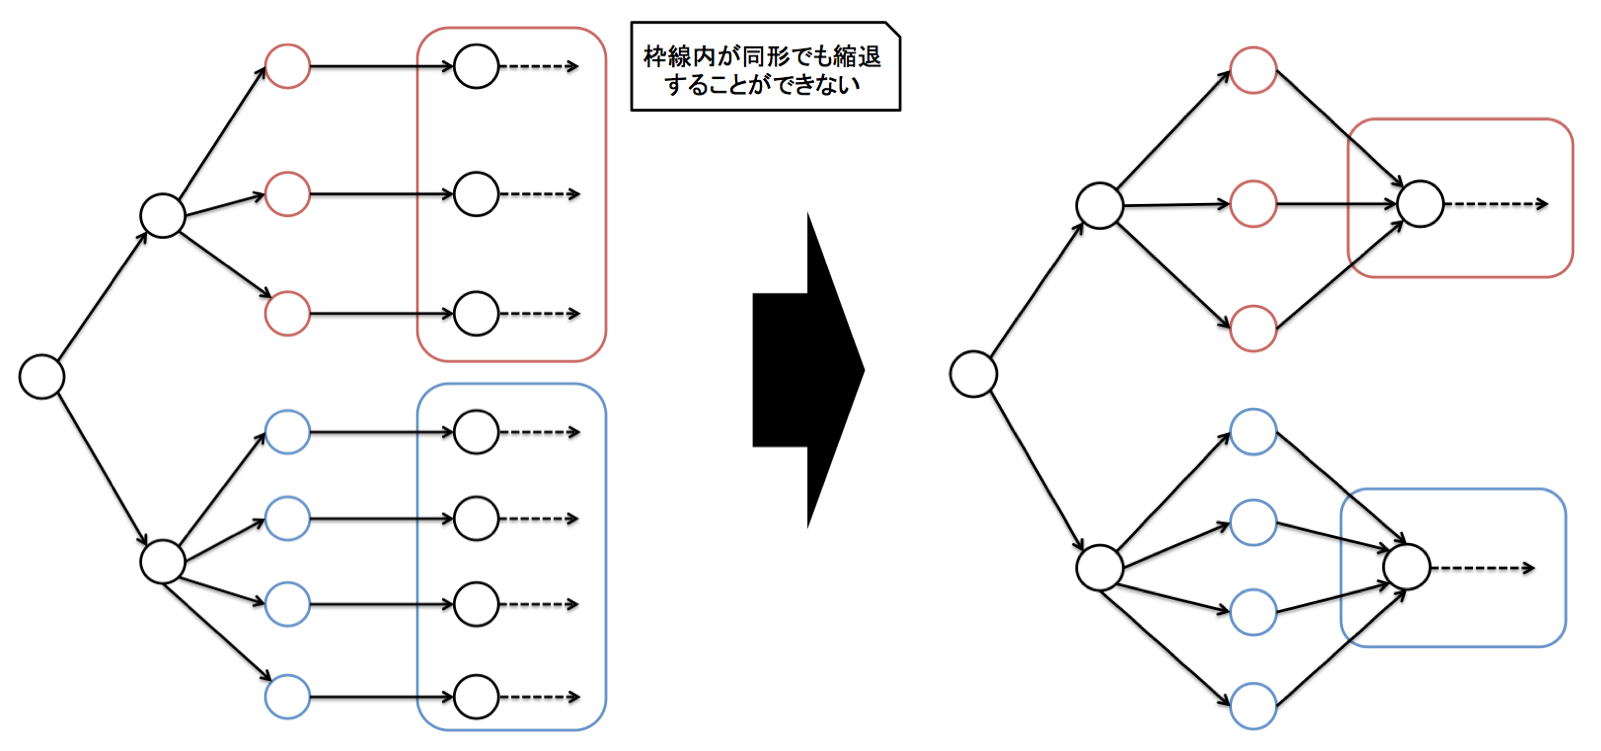
\includegraphics [clip, height=8cm]{./img/syukutai.png}
		\caption{SeqBDDを用いることで実現するデータ構造の縮退}
		\label{fig:syukutai}
	\end{center}
	\end{figure}



\section{目的}
本研究では,SeqBDDを用いることで,既存手法では不可能だった文章群をデータ構造に変換した際の末端部分の縮退を実現し,入力となる文章群をよりコンパクトな構造で表現し,可視化することでその構造の有用性を確認すること,また,構築したSeqBDDからパターンとなる語句群を抽出し評価することを目的としている.\\
 大きく分けて2つの処理を通して,文章からのパターン抽出を行う.1つは,系列データであるテキスト文章を入力としたSeqBDDを構築することである.この実現を基に,様々な節点の作成方法の検討や,節点ラベルの圧縮,余分な枝切りなどを行いデータ構造を縮退させ,よりコンパクトなデータ構造を目指す.また,SeqBDDを可視化するために,pydotと呼ばれる,GraphvizをPythonに対応させたパッケージを用いて,画像ファイルとして出力をする.
もう1つは,構築したSeqBDDからパターンを抽出する処理である.SeqBDDの構築を行う際に,よりパターンを抽出しやすいデータ構造にするために手を加えるため,比較的単純な処理によって実現することが可能となっている.\\
 これらの作業をすべて機械的に行うため,Pythonを用いてプログラムを実装する.実験には,英語の例文とイディオムを用いて頻出パターンを抽出し,それらを正解となるパターンと照合する.これらによって得られた実験結果を単純適合率,平均逆順位,平均適合率という3つの指標を用いることで評価を行う.

\section{本稿の構成}
本稿はこれ以降,4つの章によって構成されている.第\ref{text:kanrenkenkyuu}章では,本研究と深く関係する研究や論文を紹介する.
第\ref{text:teiannsyuhou}章では,本研究で提案するSeqBDDを用いた文からのパターン抽出手法を,基本となるデータ構造の説明や検討した様々な手法と共に記載している,第\ref{text:jikken_hyouka}章では,第\ref{text:teiannsyuhou}章で紹介した手法を用いて実際にパターンの抽出を行い,それによって得られた結果,および考察を示す.第\ref{text:ketsuron}章では,それらを踏まえた本研究の結論と今後の課題について述べる.




\chapter{関連研究}
\label{text:kanrenkenkyuu}
本研究と大きく関連する研究に,以下に示すパターン抽出,教師なし構文解析,用例検索が考えられる.また提案手法の準備(第\ref{text:junbi}節)のデータ構造の説明にも関連研究を記載している.


\section{パターンの抽出に関する研究}
現在,データマイニング手法を用いたパターン抽出は,コンピュータ関連の研究分野において非常に活発に行われている.その中でも,90年代前半にAgrawalらが提案した頻出集合列挙問題\cite{Agrawal:1993:MAR:170036.170072}と,その効率的な解決方法であるAprioriアルゴリズム\cite{Agrawal:1994:FAM:645920.672836}はデータマイニングの主要技術の一つとして挙げられる.Aprioriは「長さkの頻出でないパターンを含む長さk+1のパターンは頻出ではない」という仮説に基いて,ボトムアップに頻出するパターンを抽出するアルゴリズムである.
また,Aprioriのアルゴリズムを基に提案されたGSP\cite{Srikant:1996:MSP:645337.650382}と呼ばれるアルゴリズムがある.これは,Aprioriの考えをそのまま系列データに対して応用し,頻出系列を抽出するという手法である.
しかし,Apriori,GSPのアルゴリズムでは候補となるパターンが膨大な数になってしまうという欠点がある.
この欠点を改善するために,SPADE\cite{Zaki:2001:SEA:599609.599626}が提案された.SPADEは束(Lattice)という概念を用いて,候補となる系列をグループに分割し,ID-Listというデータ構造を用いることで計算コストの削減を行った.さらにSPADEを改良したSPAM\cite{citeulike:3407300}というアルゴリズムが提案された.SPAMではID-Listをビットマップを用いて表現することで,さらなる計算速度の向上を図った.\\
 一方で,候補となる系列を生成せずにデータベースを射影することによって頻出系列を抽出するPrefixSpan\cite{2001:PMS:876881.879716}と呼ばれる手法が提案された.PrefixSpanアルゴリズムを用いた簡単なパターン抽出の動作例を図\ref{fig:prefixspan}に示す.この例では,4つの系列[``abc'',\ ``aab'',\ ``acd'',\ ``cba'']から長さが1以上,出現回数が2回以上のパターンを抽出している.まず,系列を成す各文字を長さ1のパターンであると考え,それぞれの系列における出現回数を数え上げる.ここでdは出現回数の条件に反するため,パターン候補から除外され,残りの``a'',``b'',``c''について,それらの後続の文字列だけを取り出す「射影」を行う.その後,射影されたデータに対して再び出現回数を数え同様の処理を行う.``a''の射影データでは``b'',``c''がそれぞれ2回ずつ出現しているため,これらの直前の文字である``a''と結合して長さ2の``ab'',``ac''というパターンを抽出する.パターンの探索を繰り返し,新たなパターンが発見されなくなると終了する.\\

	
	%PrefixSpanの図
	\begin{figure}[htbp]
	\begin{center}
		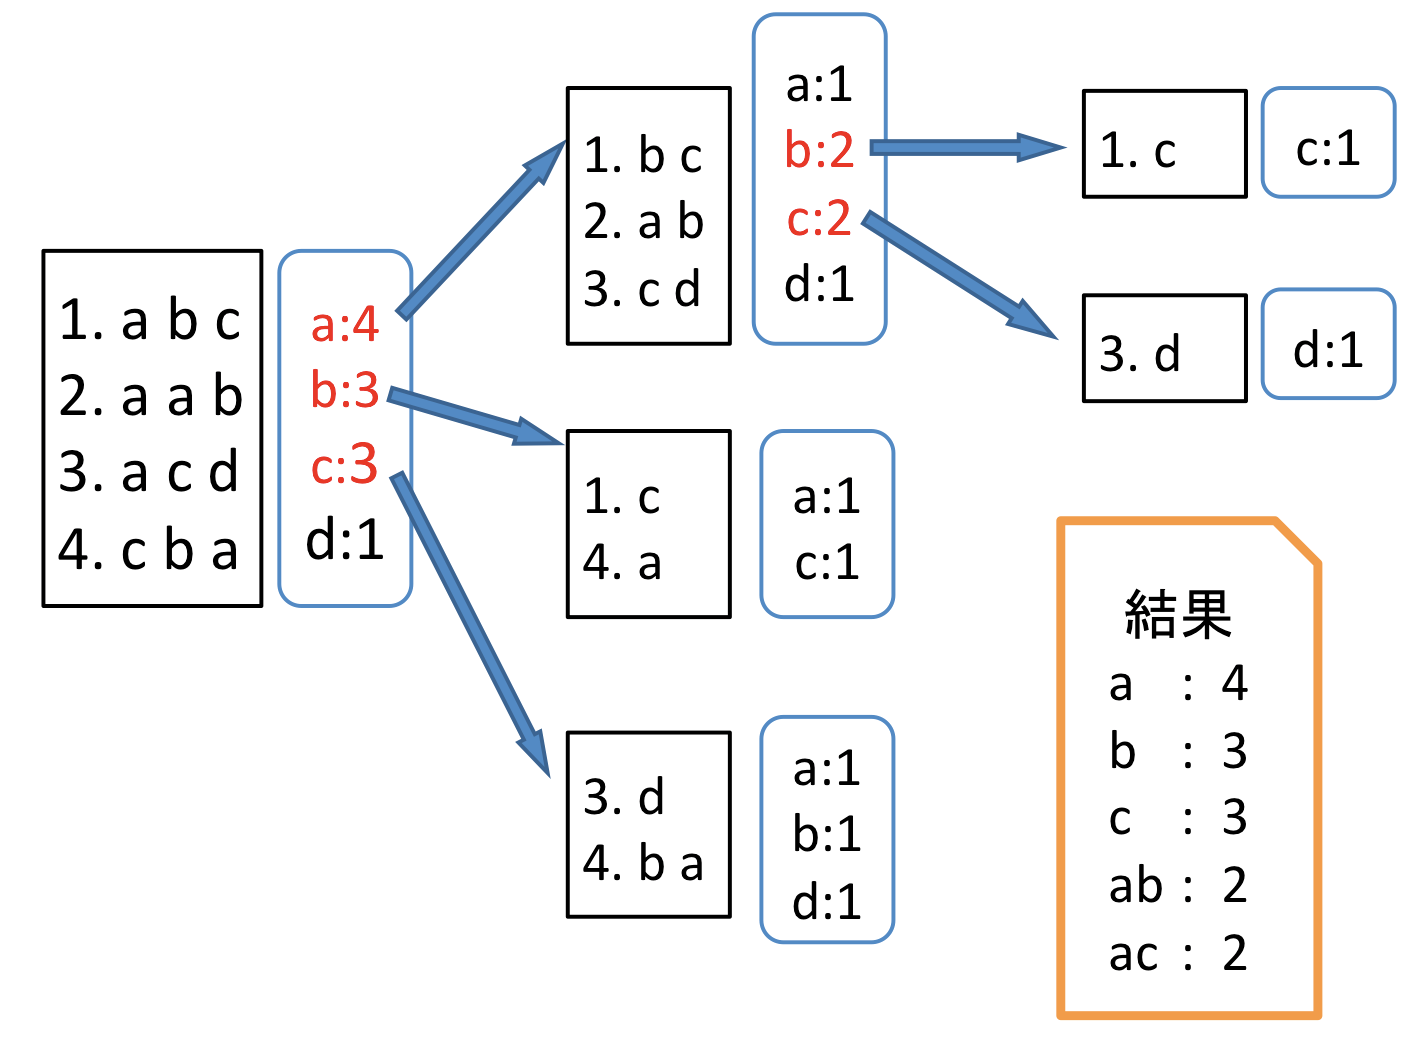
\includegraphics [clip, height=9cm]{./img/prefixspan.png}
		\caption{PrefixSpanを用いたパターン抽出例}
		\label{fig:prefixspan}
	\end{center}
	\end{figure}

 しかし,PrefixSpanを用いてテキストからパターンを抽出しようとする場合,抽出する過程で入力となるデータ毎に射影データを作成する必要があるため,多大な計算時間を必要としたり,無意味なパターンを数多く抽出してしまうという問題が存在する.また,ワイルドカード部を含むものとそうでないものを区別することが出来ないという問題もある.図\ref{fig:prefixspan}のパターン抽出例で,結果の``ac''は,入力データ``acd''では\ $<ac>$,``abc''では\ $<a*c>$\footnote{本稿では``*''はワイルドカード部を表す}という異なる出現の仕方をしているのがこれに当たる.
そこで,Modified\ PrefixSpan\cite{Kitakami:2002:MPM:646966.759862}では,頻出パターン中に存在する複数のワイルドカード領域``*''の長さを予め設定することでPrefixSpanアルゴリズムの改良を行った.\\ \\

 テキストを対象としたパターン抽出では,CRYSTAL\cite{Soderland:1995:CIC:1643031.1643069}という,注釈付きデータを含むトレーニングコーパスを用いた機械学習によって概念辞書を作成し,これを用いて生の文章からパターンの抽出を行うというシステムの研究も行われた.しかし,この手法では正確な構文規則に基づく文章からしかパターンの抽出を行うことが出来ず,柔軟性が高いとは言えない.また注釈付きデータの作成などの人的コストも高くなる.近年のネットワークやWeb技術の発達により,ネットワーク上には膨大な量のテキスト表現が増え,それに伴って煩雑な構文を含むテキストも増えた.それらに対応するために行われた研究にWHISK\cite{Soderland:1999:LIE:309497.309510}というものがある.これは,教師あり機械学習によって正規表現によるパターン抽出を行うことでより柔軟なパターンの抽出を可能とした.\\
 既存のテキストからのパターン抽出方法では,教師なし手法では正確なパターンの抽出を行うことは難しく,またパターンの抽出に重点を置くと,文章の係り受け解析などの構文解析が必要となる.本研究では,教師データを必要としないパターンの抽出を,後述するSeqBDD\cite{Loekito:2010:BDD:1851388.1851396}と呼ばれるデータ構造を用いて行う手法を提案する.


\section{教師なし構文解析に関する研究}
 教師なし構文解析の基本的なアプローチとして,PCFG(確率的文脈自由文法)に文章を変換した上で,手を加えて行く手法がある.代表的なものにKlein,Manningら\cite{Klein:2003:AUP:1075096.1075150}の手法がある.しかし,自然言語を厳密に解析するために必要となる文法は,通常,非常に複雑となってしまうため人の手によって文法を書いて与える必要がある.また,PCFGの文法カテゴリの加工処理を自動的に行う方法として,Goldwaterらの階層ディリクレ過程による単語のバイグラムモデルを用いた方法\cite{Goldwater:2006:CDU:1220175.1220260}がある.またMDL原理を用いて,文字のチャンキングを繰り返す方法\cite{MDLchang}による,統計的機械学習と考えた研究も行われている.\\
 Pattern\ Grammar\cite{pattern-grammar}では,頻出する単語に関して,前置詞や熟語,節などの言い回しをパターンとして扱い,言葉の意味を理解しようとするパターン文法が説明されている.ここでは,単語のパターンとは,単語とその意味が必ず関係づけられている構造だと定義できると述べられている.そのため,同時にかつ頻繁に出現したり,特定の言い回しであったり,明らかな意味関係が存在するような単語に関してはパターンを特定することができる.この考えを基に,本研究では教師なしの構文解析を,SeqBDDというデータ構造を用いることでパターンの抽出に拡張し,ある単語の前後の頻出単語のパターンを抽出する方法を提案する.



\section{用例検索に関する研究}
用例検索とは,ある単語を与えたときに,その単語の用例を頻度の高いものから列挙するという検索技術であり,系列マイニングの一種である.
用例検索に用いられる技術にKWIC(keyword\ in\ context)システムと呼ばれるものがある.これは,テキストからある単語を検索する際に,その前後の文脈も同時に取り出すことで検索効率を高めるという手法である.KWICを用いることで,ある単語とその単語の前後の単語を,出現頻度を用いてパターン抽出することが,単純な数え上げによって行うことができる.しかし,パターンとなりうる形や同じ単語でも異なるパターンであることを計算機自身に判別させることが難しく,ある単語の前後のパターンを抽出する技術は自動化にまで至っていない.\\
 また,用例検索を行うことのできる技術の一つに,田中らが提案したTonguen\cite{journals/ir/Tanaka-IshiiI07}と呼ばれるツールがある.これは利用者がある単語群パターンをワイルドカード部を含むパターンの枠と穴を用いて与え,そのパターンの用例のうち,穴の部分に出現する可能性の高い単語をインターネット上からリアルタイムで取得し,利用者に提示するというものである.例として,利用者が「how\ to\ *\ jet\ lag」と検索すると,ワイルドカード部である*に出現する可能性の高い単語(avoid,\ beat,\ prevent…)を得ることができる.\\
 本研究では,ある単語を与えた際に,その前後に頻出する単語のパターン抽出の自動化をSeqBDDというデータ構造を用いて実現する手法を提案する.


\chapter{提案手法}
\label{text:teiannsyuhou}
文章群からパターン抽出を行うに当たって,まず文章の構造化を行う必要がある.
本章では,系列データマイニングなどに用いられている系列二分決定グラフ(Sequence\ BDD:\ SeqBDD)を用いて文章群の構造化を行い,パターン抽出を行えるようデータ構造の調整,改変を行う手法を論じる.


\section{準備}
\label{text:junbi}
本研究で用いたデータ構造である系列二分決定グラフ(SeqBDD),およびその基礎となっているデータ構造である二分決定グラフ(BDD),ゼロサプレス型二分決定グラフ(ZDD)の説明を以下で行う.

\subsection{BDD(二分決定グラフ)}
	二分決定グラフ(Binary Decition Diagram:\ BDD)\cite{Somenzi99binarydecision}は,グラフ構造を用いて論理関数を表現する方法の一つである.ある論理関数のそれぞれの変数値について,入力(0,\ 1)に対する場合分けをそれぞれ0-枝,1-枝で表す.
	これによって,すべての変数値についての場合分けを二分決定木を用いて表すことができる.
	さらに,この二分決定木を縮約した形にするために以下の
	\begin{itemize}
		\item 冗長な節点の削除
		\item 同等な節点の共有
	\end{itemize}
	という2つの縮約規則を用いる.\\
	\ \ \ \ 1つ目の「冗長な節点の削除」について,ある節点から伸びる0-枝と1-枝の両方が同じサブグラフを指している場合,その節点と両枝を,1つの枝に置き換えても表現は同一であるため,それらを省略することができる.(図\ref{fig:bddrule}(a)を参照\footnote{図において,丸が節点,矢印がそれぞれの枝,三角形がサブグラフを表している})
	2つ目の「同等な節点の共有」について,ある2つの節点から伸びる0-枝と1-枝がそれぞれ同じサブグラフを指している場合,その節点を同等な節点とみなして,共有することでデータ構造を縮約することができる.(図\ref{fig:bddrule}(b)を参照)
	これら2つの規則を,二分決定木に対して可能な限り適用することで縮約された形の木を得ることができる.\\
	\begin{figure}[htbp]
	\begin{center}
	\begin{tabular}{c}
	%fig: binary tree
		\begin{minipage}{0.4\hsize}
			\begin{center}
			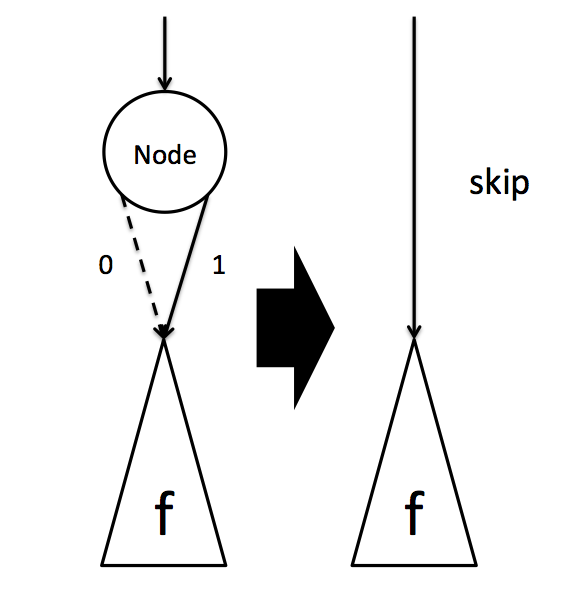
\includegraphics [clip, height=7cm]{./img/bddrule-1.png}
			\hspace{1.6cm} (a)冗長な節点の削除
			\end{center}
		\end{minipage}

	%fig: bdd
		\begin{minipage}{0.6\hsize}
			\begin{center}
			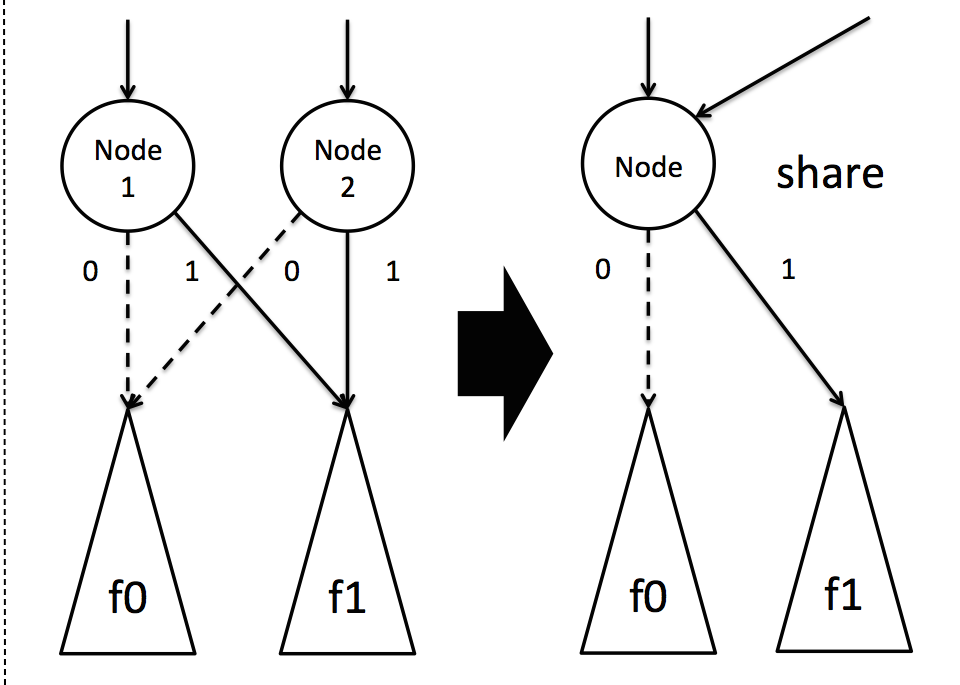
\includegraphics [clip, height=7cm]{./img/bddrule-2.png}
			\hspace{1.6cm} (b)同等な節点の共有
			\end{center}
		\end{minipage}
	\end{tabular}
	\caption{BDDの2つの縮約規則}
	\label{fig:bddrule}
	\end{center}
	\end{figure}

	\newpage
	このようにして作られる木で,変数順序が固定されているものを本論ではBDDと呼ぶ.ここで,変数順序について説明を加える.BDDにおける変数順序とは,入力となる論理関数の各変数について,予め定めておく順序関係のことを指す.この順序関係を用いて,変数順序の小さいものから節点を作成していくことになる.例えば変数順序を
	$$
	a\prec b\prec c
	$$
	と定めた場合,まず変数aに関する節点を作成し,続いてb,\ cの節点,と作成していく.\\
	 BDDは次のような性質を持つデータ構造である.基となる二分決定木のどの部分から縮約を行っても,同一の論理関数であれば出力される形は同じとなる.つまり,BDDを用いることで論理関数に対して一意に表現することができるため,等価性検証を容易に行うことができる.また,異なるBDDを入力とし,それらのBDDについての二項論理演算の計算結果であるBDDを出力する「Apply演算\cite{bryant86}」と呼ばれるアルゴリズムが考案されている.このアルゴリズムによって,データサイズが主記憶の大きさに収まる限り,論理関数同士の演算をグラフの大きさに比例する計算時間で実行することができる.\cite{Knuth:2009:ACP:1593023}\\
	\ \ BDDの具体例として,論理関数$F$について
	$$
	F(a,b,c)\ =\ abc\lor\overline{a}\overline{b}\overline{c}\\
	$$
	とした場合の,二分決定木とBDDの例を図\ref{fig:bt_bdd}に示す.この関数に対して,各入力変数に固定値を代入した際の関数の値を得たい場合,節点のラベルとなっている各変数に対して,真の場合は1-枝に,偽の場合には0-枝に進んでいき,辿り着いた終端節点の値を確認すればよい.例として,F(1,1,0)[a=1,b=1,c=0]という関数の値を得たい場合には,節点aの1-枝→節点bの1-枝→節点cの0-枝,と辿り結果として0-終端節点に行き着くため,F(1,1,0)=0を得ることができる.\\
	\ 

	\begin{figure}[htbp]
	\begin{center}
	\begin{tabular}{c}
	%fig: binary tree
		\begin{minipage}{0.66\hsize}
			\begin{center}
			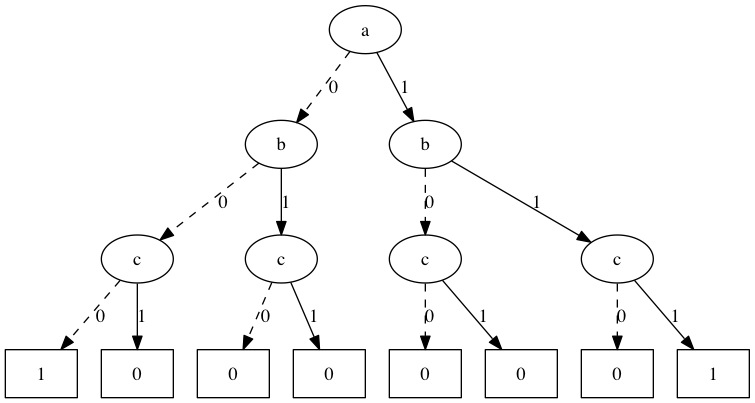
\includegraphics [clip, width=10cm, height=6cm]{./img/sample.jpeg}
			\hspace{1.6cm} (a)二分決定木
			\end{center}
		\end{minipage}

	%fig: bdd
		\begin{minipage}{0.33\hsize}
			\begin{center}
			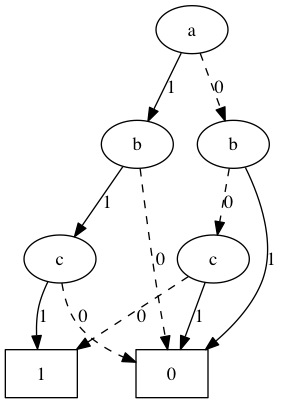
\includegraphics [clip, height=6cm]{./img/bdd_sample.jpeg}
			\hspace{1.6cm} (b)BDD
			\end{center}
		\end{minipage}
	\end{tabular}
	\caption{木による論理関数の表現例}
	\label{fig:bt_bdd}
	\end{center}
	\end{figure}


\newpage
\subsection{ZDD(ゼロサプレス型 BDD)}
	ZDD(Zero-suppressed Binary Decition Diagram:ゼロサプレス型二分決定グラフ)\cite{Minato:1993:ZBS:157485.164890}は,組み合わせ集合を効率よく表現することが出来るデータ構造である.ZDDでは,冗長な節点の削除をするための縮約規則がBDDとは異なる.BDDでは,0,1-枝が同じ節点を指している際に節点を取り除いていたが,ZDDでは1-枝が0-終端節点を指しているときのみに,その節点を冗長として取り除く.図\ref{fig:suprules}にBDDとZDDの冗長な節点の削除に対する縮約規則の比較を示す.同等な節点の共有に関する規則はBDDと同じである.\\

	 よって,ZDDの2つの縮約規則は以下のようになる.
	\begin{itemize}
		\item 1-枝が0-終端節点を直接指している節点の削除
		\item 同等な節点の共有
	\end{itemize}

	ZDDにおける根から終端節点への1つの経路は,1つの組み合わせを表している.1-終端節点に辿り着く経路の1-枝を持っている節点のラベル(変数)の集合を,1つの組み合わせ集合として扱うことができる.図\ref{fig:zdd_sample}に,図\ref{fig:bt_bdd}と同じ論理関数を表したZDDを示す.\\


	% 縮約規則比較図
	\begin{figure}[htbp]
	\begin{center}
	\begin{tabular}{c}
	%fig: binary tree
		\begin{minipage}{0.5\hsize}
			\begin{center}
			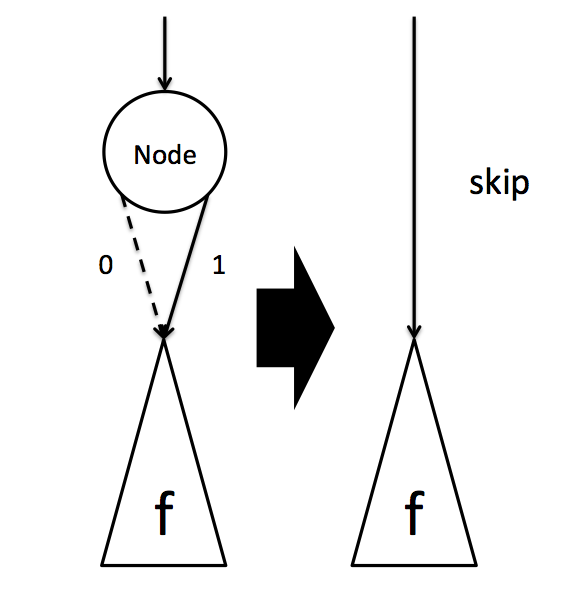
\includegraphics [clip, width=6cm]{./img/bddrule-1.png}
			\hspace{1.6cm} (a)BDDの節点削除規則
			\end{center}
		\end{minipage}

	%fig: bdd
		\begin{minipage}{0.5\hsize}
			\begin{center}
			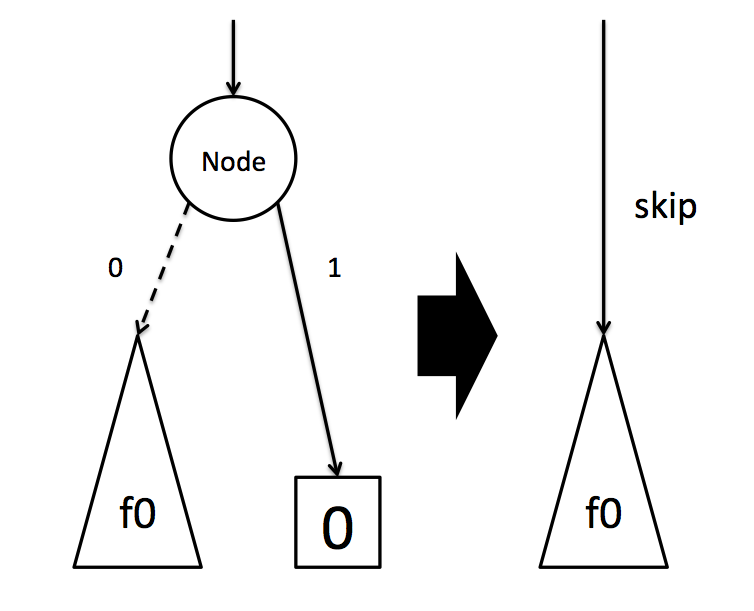
\includegraphics [clip, height=6cm]{./img/zddrule.png}
			\hspace{1.6cm} (b)ZDDの節点削除規則
			\end{center}
		\end{minipage}
	\end{tabular}
	\caption{BDDとZDDの縮約規則の比較}
	\label{fig:suprules}
	\end{center}
	\end{figure}


	%zdd例
	\begin{figure}[htbp]
	\begin{center}
		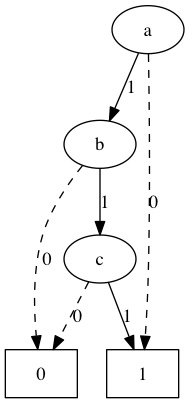
\includegraphics [clip, height=9cm]{./img/zdd_sample.jpeg}
		\caption{論理関数abc$\lor\overline{a}\overline{b}\overline{c}$のZDD}
		\label{fig:zdd_sample}
	\end{center}
	\end{figure}


	論理関数F(a,b,c)=abc$\lor\overline{a}\overline{b}\overline{c}$を組み合わせ集合と考えた場合,集合Sとすると
	$$
	S=\{\{\varepsilon\},\ \{abc\}\}
	$$
	と表すことができ,それぞれの組み合わせについて真ならば集合に含まれ,偽ならば集合には含まれないことが分かる.変数に値を代入して関数値を得たい場合は,BDDと同様に節点(変数)について各枝を辿っていき,終端節点の値を調べる.また図\ref{fig:zdd_sample}の例では,経路によって出現しない変数が存在する(例として,a=1,b=0の場合,cの節点が出現しない)が,これは例に沿うと,aが集合に含まれ,bが集合に含まれない組み合わせには,cは必ず出現しない,ということを表している.よって,組み合わせ集合に出現しない変数については節点が削除されるため,BDDと比べると,組み合わせ集合を表現することに特化していると言える.またZDDも,BDDと同様に表現の一意性を持っており,Apply演算\cite{bryant86}を用いることによって,2つのZDD同士の集合演算を行うことも可能である.\\
	 しかし,ZDDは組み合わせ集合に特化しているデータ構造であるため,変数が複数出現(\{aa,aab,abb\})したり,順序違い(\{ab,ba\})などは扱うことが出来ない.変数毎に符号化を行うことで,ZDDで系列集合を表現する方法\cite{conf/jsai/KuraiMZ06}も考案されている.この方法であれば,同じ変数でも出現位置によって符号を変える($a_{1}a_{2}a_{3}など$)ことで異なる変数として扱うことができるため,組み合わせ集合によって系列集合を表現することは可能になる.しかし,系列の最大長とアルファベットのサイズの積に比例して変数の数が増加したり,出現位置の微差でも部分系列の共有ができなくなる\cite{minato:recently-bdd}という欠点があるため,あまり効率のよい方法とは言えない.


	\newpage
	\subsection{SeqBDD(シーケンス型 BDD)}
	\label{seqbdd}
	SeqBDD\cite{Loekito:2010:BDD:1851388.1851396}は,ZDDでは効率よく表現出来なかった,系列集合に対して最適化されたデータ構造であり,伝住ら\cite{suffixdd}によって``Suffix-DD''と呼ばれるSeqBDDを用いた部分文字列索引の構築などの系列データマイニングに利用されている.\\
	 BDD,ZDDでは,各親の節点と子の節点に対して変数順序と呼ぶ,各変数間に定めた順序付けが存在した.これに対してSeqBDDは,変数の順序付けを0-枝のみに適用し,1-枝側についてはその順序付けの制約を外した.この制約緩和によって,各変数について1つの経路で複数回の出現や変数の逆順を許すことになり,系列集合を効率よく表現することが出来る.図\ref{fig:zdd-seqbdd}に変数$\Sigma=(a,b,c)$に対して,変数順序を$a\prec b\prec c$とした場合のZDDとSeqBDDの変数順序の例を示す.ZDDではすべての節点について変数順序が定められているため,すべての節点の変数はその親の節点の変数よりも大きい変数順序の変数をラベルとして持っている.一方,SeqBDDでは前述した通り,1-枝側での変数順序の制約が存在しないため,子の節点の変数が親の節点の変数より小さいことを許している.例えば,bの変数の節点の1-枝側にはbよりも変数順序が小さく,すでに節点が存在するaについて再び節点が作成されている.
	\begin{figure}[htbp]
	\begin{center}
	\begin{tabular}{c}
	%fig: binary tree
		\begin{minipage}{0.5\hsize}
			\begin{center}
			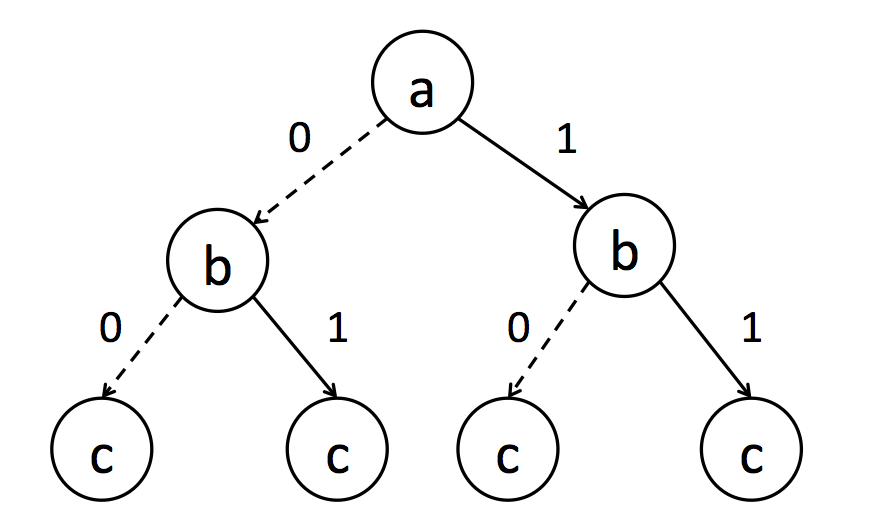
\includegraphics [clip, height=5.2cm]{./img/zdd_num.png}
			\hspace{1.6cm} (a)ZDD
			\end{center}
		\end{minipage}

	%fig: bdd
		\begin{minipage}{0.5\hsize}
			\begin{center}
			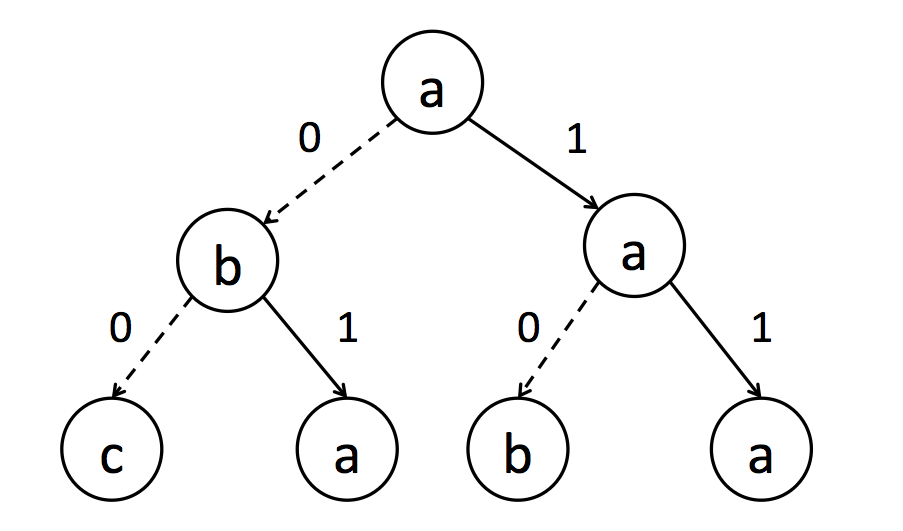
\includegraphics [clip, height=5.2cm]{./img/seqbdd_num.png}
			\hspace{1.6cm} (b)SeqBDD
			\end{center}
		\end{minipage}
	\end{tabular}
	\caption{ZDDとSeqBDDの変数順序について}
	\label{fig:zdd-seqbdd}
	\end{center}
	\end{figure}


	\newpage
	SeqBDDでは,1つの経路が1つの系列を表しており,最終的に1-終端節点に到達した場合には,その系列が集合に含まれるということになる.
	例として,系列集合
	$$f = \{aaa,\ aca,\ ba,\ bc\}$$
	に対するSeqBDDを図\ref{fig:seqbdd_sample}に示す.変数順序は$a\prec b\prec c$とする.本論ではこれ以降提示する図において,0-終端節点の表示を省略し,1-枝を実線,0-枝を破線で表す.\\
	 ここでLoekitoら\cite{Loekito:2010:BDD:1851388.1851396}によって提案されたSeqBDDを構築するアルゴリズムの擬似コードを{\bf Algorithm\ref{alg:build_seqbdd}},および{\bf Algorithm\ref{alg:getnode}}に示す.
	SeqBDDの構築は,まず頂点となる節点からそれぞれの系列の先頭文字が節点の変数で始まるかどうか,を場合分けして枝別れを行う.図\ref{fig:seqbdd_sample}を参考にすると,まず変数順序が最小である変数aについて,系列集合$f$の各系列をaで始まるものとそうでないものに分けて節点$N=node(a,N_{a},N_{\overline{a}})$を作成する.
	ここで$node(a,N_{a},N_{\overline{a}})$は,文字{\bf a}を変数として持ち,1-枝が$N_{a}$,0-枝が$N_{\overline{a}}$を指す節点を示す.
	$N_{a}$に含まれる系列集合は,先頭文字を削除した系列を追加する.図\ref{fig:seqbdd_sample}の場合,
	
	$$
	N_{a}=\{ca,aa\},\ N_{\overline{a}}=\{ba, bc\}
	$$
	
	となる.
	この処理をAlgorithm\ref{alg:build_seqbdd}では,7行目で変数$x$に変数順序が最小の文字を入れ,8行目からのforループを用いて各系列を$x$で始まる系列とそうでない系列に分けて,Algorithm\ref{alg:getnode}に示すGetnodeという関数を用いて節点の作成を行っている.
	続く文字に対しても同様の処理を再帰的に行い,最終的に場合分けをした際に\{$\varepsilon$\}となるとき1-終端節点を,Φとなるときには0-終端節点を指すように枝を作成する.Algorithm\ref{alg:build_seqbdd}では,2行目および4行目によって終端節点かどうかの判定を行っている.
	図\ref{fig:seqbdd_sample}の例では,左下に位置するcの節点に対して場合分けをした場合,作成される節点$node(c,N_{c},N_{\overline{c}})$では,
	
	$$
	N_{c}=\{\varepsilon\},\ N_{\overline{c}}=\Phi
	$$
	となるため,1-枝は1-終端節点を,0-枝は省略しているが0-終端節点を指している.\\

	 また,Algorithm\ref{alg:getnode}に示した$Getnode$のアルゴリズムは,SeqBDD(ZDDと同様)の縮約規則である
	\begin{itemize}
	\item 1-枝が0-終端節点を指している場合節点を削除
	\item 同一な節点の共有
	\end{itemize}
	を行いながら,入力として与えられる変数と2つの枝先となるサブグラフを指す節点の作成を行う.
	節点の共有を実現するために,ハッシュテーブルを用いて演算結果を管理しておき,同一な節点が既に作成済みである場合には新たに節点を作らず,既存の同一な節点を返すようにしている.


	\begin{figure}[htbp]
	\begin{center}
		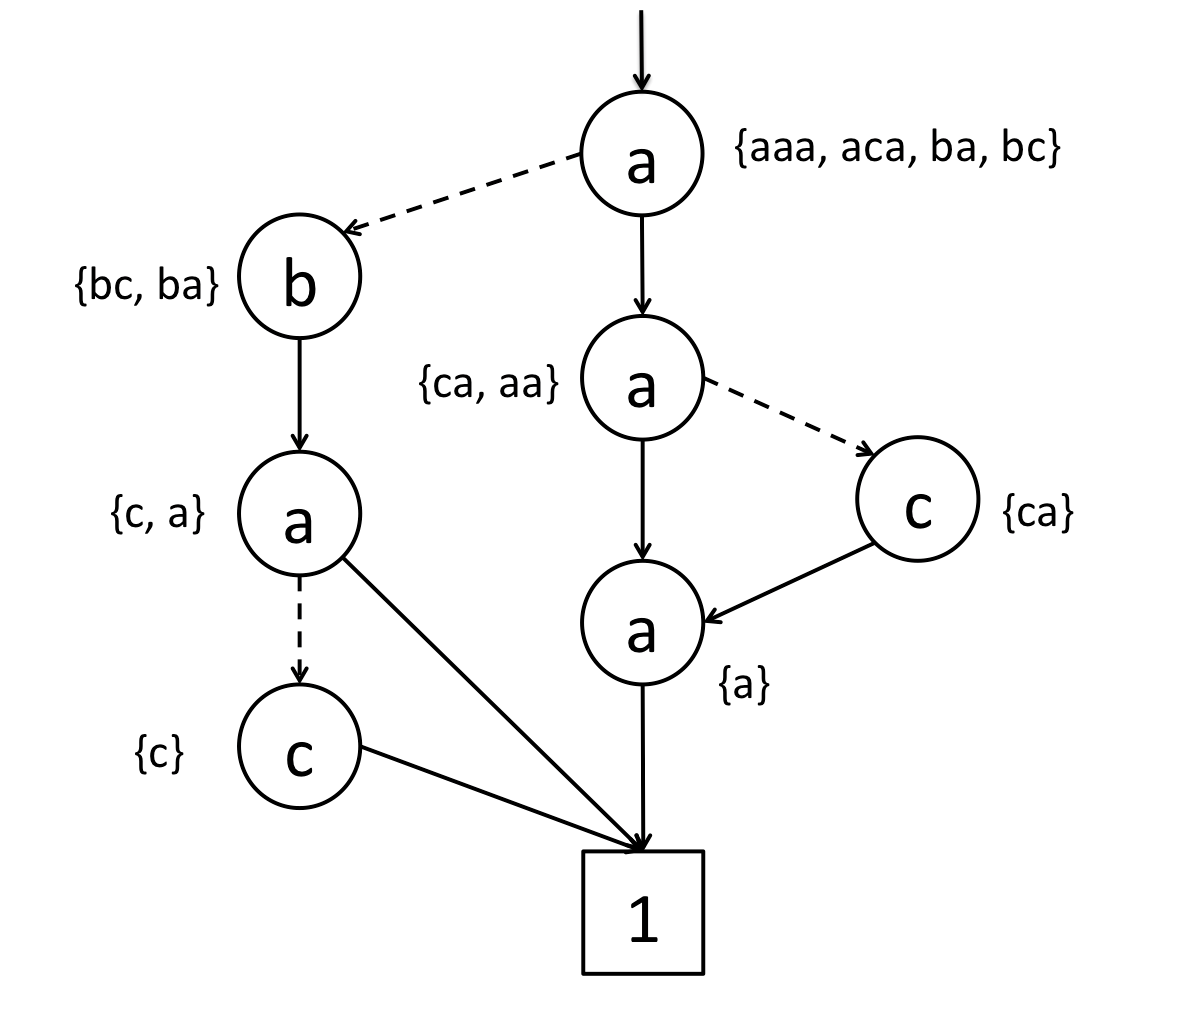
\includegraphics [clip, width=14cm]{./img/seqbdd_sample.png}
		\caption{SeqBDDの例}
		\label{fig:seqbdd_sample}
	\end{center}
	\end{figure}


%アルゴリズム	
\begin{algorithm}
		\caption{Build SeqBDD}
		\label{alg:build_seqbdd}
		\begin{algorithmic}[1]
		\REQUIRE $f(系列集合)$
		\ENSURE	 $SeqBDD$
			\STATE sort($f$)
			\IF [空列(1-終端節点)の場合] {$f = \{ \lambda \}$} 
			\RETURN \TRUE
			\ELSIF [空集合(0-終端節点)の場合] {$f=\Phi$} 
			\RETURN \FALSE
			\ENDIF
			\STATE $x \leftarrow f[0][0]$	\COMMENT{系列集合のうち変数順序が最小の先頭文字を$x$とする}
			\FOR {$i=0$ to $|f|$}
				\IF {$f[i]=x$}
					\STATE $f_{x}$.append($f[i][0]$)
				\ELSE
					\STATE $f_{\overline{x}}$.append($f[i][0]$)
				\ENDIF
			\ENDFOR
			\STATE $R \leftarrow$ Getnode($x,\ Build SeqBDD(f_{x}),\ BuildSeqBDD(f_{\overline{x}})$)
			\RETURN $R$

		\end{algorithmic}
		\end{algorithm}

		% getnode
		\begin{algorithm}
		\caption{Getnode}
		\label{alg:getnode}
		\begin{algorithmic}[1]
		\REQUIRE $top, P_{0}, P_{1}$
		\ENSURE $tree$ \COMMENT{node with two subgraph $P_{0}$ and $P_{1}$}
			\IF {$P_{1} = \Phi$}
				\RETURN $P_{0}$	\COMMENT{1-枝が0-終端節点を指していたら節点を削除}
			\ENDIF
			\STATE $P \leftarrow$ search\ a\ node\ with\ $<top, P_{0}, P_{1}>$ in $uniqtable$
			\IF {$P\ exist$}
				\RETURN $P$ \COMMENT{既に同形のサブグラフを作成済みの場合共有}
			\ENDIF
			\STATE $P \leftarrow$ newnode$(top,P_{0},P_{1})$
			\STATE $uniqtable<top,P_{0},P_{1}> \leftarrow P$
			\RETURN $P$
		\end{algorithmic}
		\end{algorithm}


\newpage
\section{文を入力としたSeqBDDを構築するための工夫}
\label{text:build_seqbdd}
	\ref{seqbdd}で説明した既存のSeqBDDの構築法を基に,文章を入力としたSeqBDDの構築を行う.言語はPythonを用いて実装し,出力にはPydotというモジュールを用いて画像出力を行っている.


	\subsection{文字,単語による節点の作成}
	SeqBDDを用いて文を構造化しようとする際に,まず節点のラベルとなる各変数について定めなければならない.本節では,まず文の各文字を変数として考えた場合のSeqBDDの構築を行う.\\
	 例として,入力$f$となる文を,
	\begin{eqnarray*}
	\label{text:stream_str}	
	f=[\ 私は中学生です,\ 私は大学生です,\ 私は小学生です,\\ 私は学生です,\ 私は学生ではない]
	\end{eqnarray*}
	とした場合に構築されるSeqBDDを図\ref{fig:seqbdd_graph1}(a)に示す\footnote{これ以降のSeqBDDの出力画像は,1-枝を赤線,0-枝を黒線で示し,また0-終端節点は省略する.}.
	ここで同一節点間に,枝が複数現れているサブグラフが見受けられるが,これはSeqBDDの縮約規則である「同等な節点の共有」を分かり易く示したものである.\\
	 節点を文字としてSeqBDDを構築した場合,入力となる系列集合の各変数間の変数順序が問題として挙がった.変数順序はSeqBDDを構築する際に,各節点の作成順序を定めるものとなるが,この順序によって木が理想形とならずパターンの発見が難化した.簡単な具体例を図\ref{fig:seq_str_miss}に示す.入力は
	$f=[小学生, 学生]$の2文である.この場合,理想形は根となる節点のラベルが「``小''」で,「``学'',``生''」という節点を共有して,「``学生''」というパターンを得ることが理想である.しかし,Pythonの内部関数を用いてソートを行うと「``小''」よりも「``学''」のほうが変数順序が小さいため,結果として「``生''」の節点しか共有されない.前に示した\ref{fig:seqbdd_graph1}(a)の小学生,学生の枝分かれの部分でも確認することができる.\\
	 これを踏まえて次に,入力となる文に形態素解析を行って単語毎に区切り,節点を単語としたSeqBDDを構築した.例を図\ref{fig:seqbdd_graph1}(b)に示す,入力は図\ref{fig:seqbdd_graph1}(a)と同じである.

	\begin{figure}[htbp]
	\begin{center}
		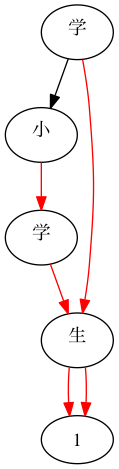
\includegraphics [clip, width=1.8cm]{./img/seqbdd_no_sort.png}
		\caption{変数順序によるパターン発見の難化}
		\label{fig:seq_str_miss}
	\end{center}
	\end{figure}


	\begin{figure}[htbp]
	\begin{center}
	\begin{tabular}{c}
	%fig: binary tree
		\begin{minipage}{0.3\hsize}
			\begin{center}
			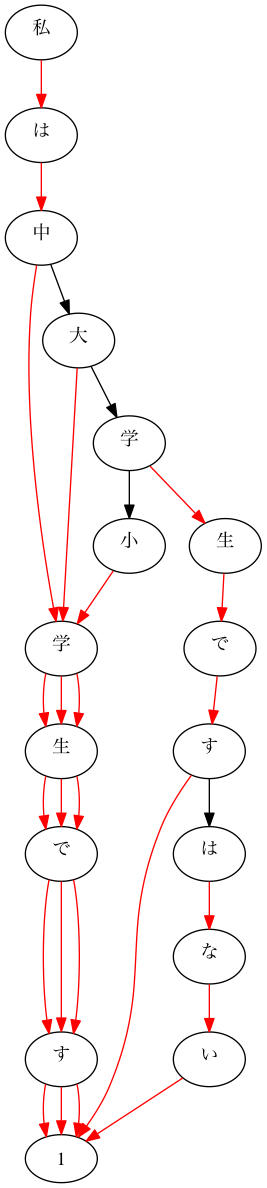
\includegraphics [clip, height=17cm]{./img/example_graph_word1.png}
			\hspace{1.6cm} (a)文字を節点
			\end{center}
		\end{minipage}

	%fig: bdd
		\begin{minipage}{0.4\hsize}
			\begin{center}
			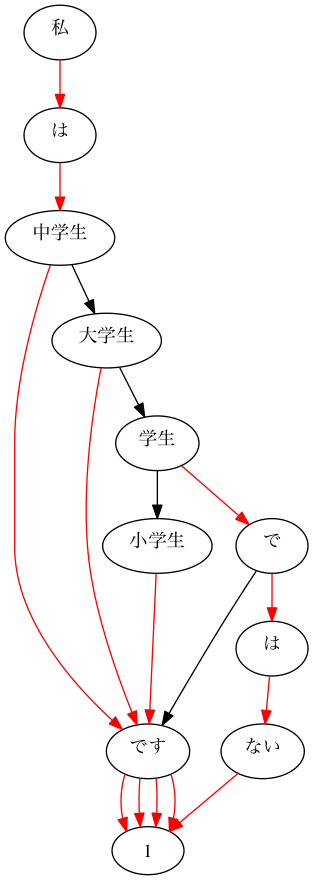
\includegraphics [clip, width=5cm]{./img/example_graph_word2.png}
			\hspace{1.6cm} (b)単語を節点
			\end{center}
		\end{minipage}
	\end{tabular}
	\caption{構築したSeqBDDの例}
	\label{fig:seqbdd_graph1}
	\end{center}
	\end{figure}

	\newpage
	文を単語列に区切るために,「MeCab\footnote{http://mecab.googlecode.com/svn/trunk/mecab/doc/index.html}」という形態素解析エンジンを用いた.単語毎に節点を作成することで,文をソートする際の参照する変数(文字)が増えるため,前述した変数順序によるパターン発見の問題を大幅に改善することができた.\ref{fig:seqbdd_graph1}(b)を見ると,(a)よりもコンパクトな表現になっているのが分かる.本来は,(小,中,大)といった文字で枝分かれし,[``学生'',``です'']という節点を共有することが理想である.これはより詳細な形態素解析データを用いて節点の作成を行うことで可能となるが,今回は単語による節点の作成を主としていないため省略した.\\
	 単語で節点の作成を行ってパターンを取得しようとする場合,単語が完全に一致していないと節点の共有が出来ないため,容易にパターンを得ることが出来ない.そこで,節点の共有判定の緩和を目的とした新たな節点の作成方法として次節\ref{text:seq_with_parts}で述べる,単語に品詞情報を付与した,単語の品詞による節点の作成を行う.

	
	\subsection{品詞による節点の作成}
	\label{text:seq_with_parts}
	入力となる文を単語列に区切り,品詞情報を単語ごとに付与して,単語の品詞を節点の変数としてSeqBDDの構築を行う.また,入力となる文章は英語を対象とした.\\
	 入力となる文を,
	\begin{eqnarray*}
	f=[\ I\ am\ a\ high\ school\ student&,& I\ was\ a\ high\ school\ student,\\
	\ \ \ \ \ \ \ You\ are\ a\ high\ school\ teacher&,& I\ am\ a\ high\ school\ teacher,\\
	\ \ \ \ \ \ \ He\ is\ a\ high\ school\ student\ ]&&
	\end{eqnarray*}

	とした場合の,節点を単語および品詞で作成したSeqBDDの比較を図\ref{fig:seqbdd_graph2}に示す.文の単語列への分割,品詞情報の付与は「NLTK\footnote{http://www.nltk.org}」という形態素解析エンジンを用いた.

	\begin{figure}[htbp]
	\begin{center}
	\begin{tabular}{c}
	%fig: binary tree
		\begin{minipage}{0.4\hsize}
			\begin{center}
			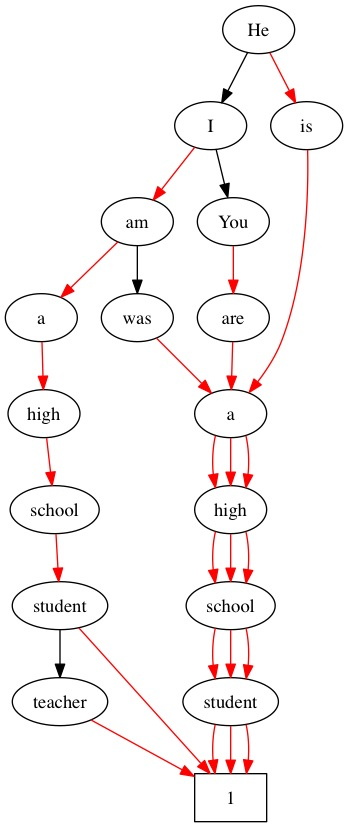
\includegraphics [clip, width=5cm]{./img/seq_word.jpeg}
			\hspace{1.6cm} (a)単語を節点
			\end{center}
		\end{minipage}

	%fig: bdd
		\begin{minipage}{0.6\hsize}
			\begin{center}
			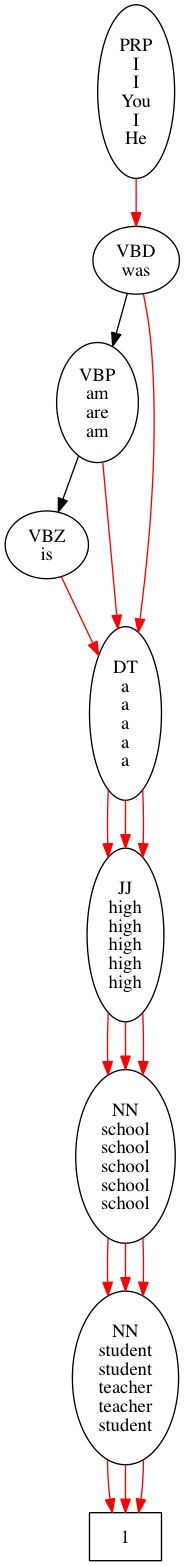
\includegraphics [clip, height=19cm]{./img/seq_parts.jpeg}
			\hspace{1.6cm} (b)品詞を節点
			\end{center}
		\end{minipage}
	\end{tabular}
	\caption{節点を単語/品詞で作成したSeqBDDの比較例}
	\label{fig:seqbdd_graph2}
	\end{center}
	\end{figure}

	\newpage
	品詞毎に節点を作成する際に,節点の変数は節点のラベル1行目に表示されている品詞(例:PRP,VBPなど)とし,その品詞が入力ではどの単語に当たるかを節点のラベルの2行目以降に例として表示している.節点を品詞毎に作成することで,節点の変数となり得る数が単語に比べて非常に少なくなるため,サブグラフの共有判定の緩和に繋がり,またパターン抽出の易化に繋がる.図\ref{fig:seqbdd_graph2}(a)の単語で節点を作成した場合には共有されない部分が,(b)の品詞の場合では改善されていることが見て取れる.


	\subsection{枝のランク付け}
	\label{text:rank_edge}
	作成したSeqBDDに対して枝にランク(重み)を付けることで,各経路,および各枝の出現頻度を調べることができるようになる.ランク付けの方法は
	\begin{itemize}
		\item 入力となる各文章に対して,その文章に対応する経路の枝のランクをすべて+1する
	\end{itemize}
	という単純なアルゴリズムを採用している.この方法によってランク付けされたSeqBDDを更に第\ref{text:seq_arrange}節で説明する方法によって,パターンを抽出し易い形へと調整する.\\

%
\newpage
\section{SeqBDDの調整とパターンの抽出}
\label{text:seq_arrange}
前節までに,品詞毎に節点を作成しランク付けを行ったSeqBDDに対して,更にパターンを抽出し易い構造になるようにデータ構造の改良を行った.

	\subsection{親を共有する0-枝の削除}
	SeqBDDの構造上0-枝は必然的に出現するが,0-枝は可能な限り数が少ない構造の方が,視覚的にわかりやすく,またパターンの抽出を行い易い.
	このとき,{\bf 根以外の節点を枝元とする0-枝}は,その0-枝を根の方に辿って行き,初めに通る1-枝の枝元の節点から1-枝を伸ばすことで,枝の置換が可能である.図\ref{fig:seqbdd_graph2}(b)と同様の入力に対してランク付け,および0-枝の削除を行ったものを図\ref{fig:remove_0-edge}に示す\footnote{品詞の後ろの括弧内の数字は根となる節点からの距離を示す}.
	この処理を行うことで,根を枝元とする0-枝以外はすべて1-枝に置き換えることができるため,文章をSeqBDDで表す際に,より簡潔なデータ表現として扱うことが可能となる.

	%0-枝削除
	\begin{figure}[htbp]
	\begin{center}
		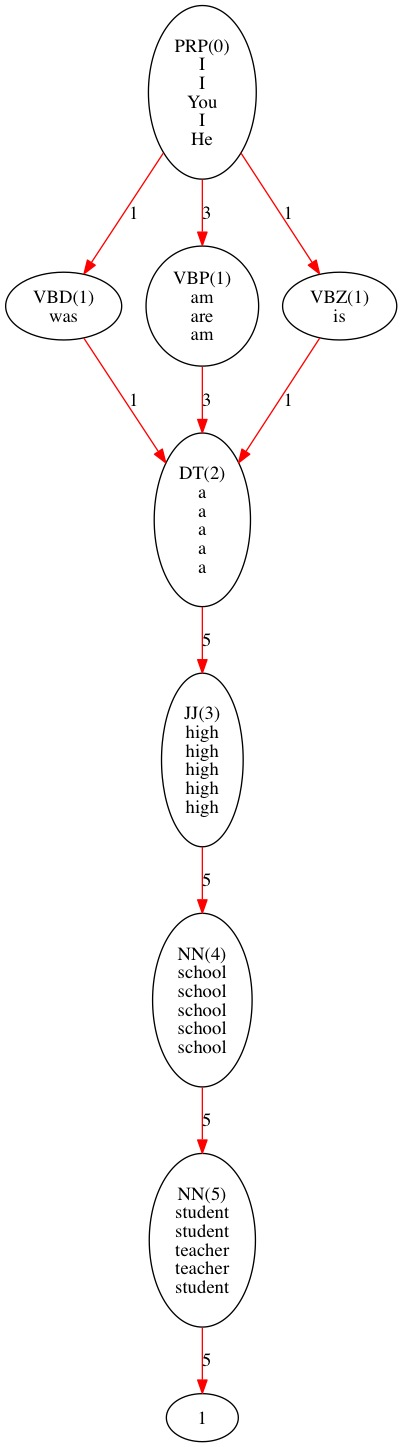
\includegraphics [clip, width=5cm]{./img/remove_0-edge.jpeg}
		\caption{0-枝の削除}
		\label{fig:remove_0-edge}
	\end{center}
	\end{figure}

	\subsection{ランクによる枝の削除}
	SeqBDDからパターンを抽出する前処理として,次に「枝切り」の処理を行う.ここで行う枝切りのアルゴリズムを{\bf Algorithm\ref{alg:remove_rank1}}に示す.\\
	 {\bf ランクが1の枝をすべて削除し,その後どの枝の枝先にもなっていない節点を始点とするサブグラフの削除}という方法で枝切りを行っている.
	枝切りを行うことで出現頻度の少ない枝,節点を削除し,出現頻度の高い節点のみにフィルタリングすることができ,データサイズの圧縮にも繋がることでパターン抽出をより高速に行うことが可能となる.\\
	\\

	%remove_rank1
	\begin{algorithm}
	\caption{Remove Rank1-edge}
	\label{alg:remove_rank1}
	\begin{algorithmic}[1]
	\REQUIRE $SeqBDD$
	\ENSURE  $SeqBDD\ removed\ rank−1edge$
		\FORALL {$edge \in SeqBDD$}
			\IF {$edge.label = 1$}
				\STATE ${\bf remove}\ edge\ {\bf from}\ SeqBDD$	\COMMENT{ランクが``1''の枝をすべて削除}
			\ENDIF
		\ENDFOR
		\STATE	$RemoveNodes \leftarrow Node\ (which\ is\ not\ used\ as\ the\ destination\ of\ edge)\in SeqBDD$
		\FORALL {$n \in RemoveNodes$}
			\STATE ${\bf remove}\ Subgraph\ that\ starts\ with\ n\ {\bf from}\ SeqBDD$\\
			\COMMENT{どの枝の枝先にもなっていない節点以下のサブグラフをすべて削除}
		\ENDFOR
		\RETURN $SeqBDD$
	\end{algorithmic}
	\end{algorithm}


	\subsection{節点ラベルの圧縮}
	\label{text:assyuku}
	品詞付きの単語でSeqBDDを構築した際に,節点となっている品詞をパターンとして抽出すると,品詞列のパターンしか取ることが出来ない.そこで,節点のラベルに含まれていた単語例を用いてパターンを抽出することを考える.節点のラベルとなっている品詞+単語列のうち,単語列の各単語について,次の式
	\begin{equation}
	\label{exp:sup_node}
	閾値\ x\ ≦\ (単語の出現回数)\ /\ (節点の単語例の総数)
	\end{equation}
	を満たす単語$W$が存在する場合には,その節点のラベルを品詞+$W$という表示にする.図\ref{fig:sup_node}に閾値を$x=0.6$としたときの圧縮例を示す.INで表される前置詞の節点について,``about''という単語が閾値を超えているため,節点のラベルの表示を変更する.\\

	%ノード圧縮
	\begin{figure}[htbp]
	\begin{center}
		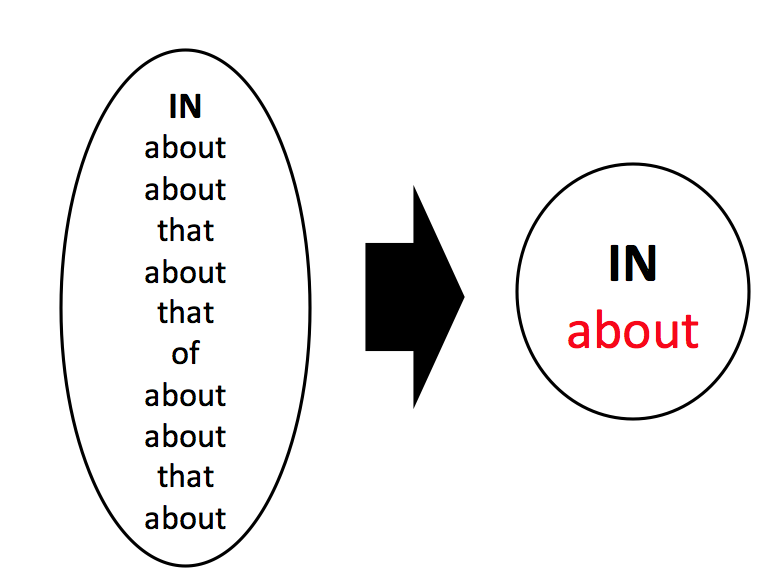
\includegraphics [clip, width=8cm]{./img/sup_node.png}
		\caption{節点ラベルの圧縮例}
		\label{fig:sup_node}
	\end{center}
	\end{figure}	

	\newpage
	\subsection{パターンの抽出方法}
	前節までの方法で構築されたSeqBDDからパターンを抽出する方法を説明する.例として,図\ref{fig:seqbdd_graph2}と同じ入力からのパターン抽出を考える.まず,前節までに説明した処理を行ったあとのSeqBDDで,式(\ref{exp:sup_node})の閾値を$x=0.6,\ 0.65$としたものを,それぞれ図\ref{fig:seq_get_pattern}\ (a),\ (b)に示す.\\
	(a)の場合,すべての節点にラベルの圧縮処理がされているため,パターン${\bf P}$は
	$$
	P\ =\ {\bf I\ am\ a\ high\ school\ student}
	$$
	と抽出する.一方,(b)のように圧縮されていない節点を含む場合には,
	$$
	P\ = \ 【*/PRP】\ \ {\bf am\ a\ high\ school}\ \ 【*/NN】
	$$
	というように圧縮されていない節点を,*を用いて【*/(品詞)】として表現することで{\bf ワイルドカード}部として扱ってパターンとする.\\
	\begin{figure}[htbp]
	\begin{center}
	\begin{tabular}{c}
	%fig: binary tree
		\begin{minipage}{0.5\hsize}
			\begin{center}
			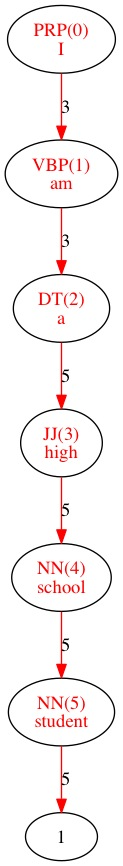
\includegraphics [clip, height=16cm]{./img/pattern_test1.jpeg}
			\hspace{1.6cm} (a)閾値$x=0.6$
			\end{center}
		\end{minipage}

	%fig: bdd
		\begin{minipage}{0.5\hsize}
			\begin{center}
			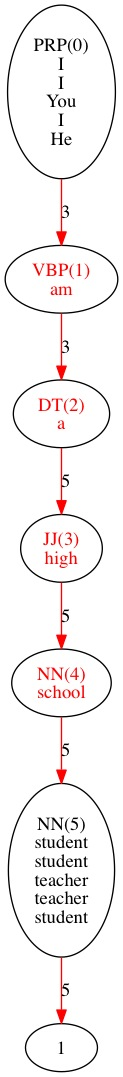
\includegraphics [clip, height=16cm]{./img/pattern_test2.jpeg}
			\hspace{1.6cm} (b)閾値$x=0.65$
			\end{center}
		\end{minipage}
	\end{tabular}
	\caption{パターン抽出を行うSeqBDDの例}
	\label{fig:seq_get_pattern}
	\end{center}
	\end{figure}


%実験
\chapter{実験と評価}
\label{text:jikken_hyouka}
\section{実験概要}
構築したSeqBDDからパターンを抽出するに当たり,本研究において目的とするパターンを「ある単語が与えられたときに,その単語の前後に現れる単語列の中で頻度の高い単語(品詞)列」であると定める.

	\subsection{実験方法}
	今回は,目的とするパターンのうち特に「与えられる単語の後ろに出現しやすい単語列」に注目をした.与えられる単語(以後``Query''と呼ぶ)が出現する文章をコーパスから抜き出し,文章をQueryの前で区切り,それ以降の単語列を入力としてSeqBDDを構築する.これにより,根となる節点のラベルは常にQueryとなり,Queryに続く可能性の高いパターンを抽出することが可能となる.\\
	 本実験では,以下に示す実験工程を行って最終的に得られるパターンとそのパターンに対応する正解データを比較することによりパターンの照合を行う.SeqBDDの構築方法については第\ref{text:build_seqbdd}章にて論じている提案手法を用いる.正解データは英語のイディオム,Queryはイディオムの先頭語,としてSeqBDDの構築を行い,得られるイディオムのパターンと正解パターンが一致するかどうかを検証する.

	\begin{itembox}[l]{実験工程}
	\label{jikken_tejun}
	\begin{enumerate}
		\item ``Query''となるイディオムを決める
		\item Query全体を含む文章をコーパスより抜き出し,Query前で文章を区切る
		\item 一定数の文章が集まったイディオムについてのみ次の工程に移る
		\item 工程(2)までに出来た文章を入力としてSeqBDDを構築
		\item パターンとして抽出できる単語列をランク順に列挙し,パターン候補とする
		\item パターン候補と正解データを比較し,評価を行う.
	\end{enumerate}
	\end{itembox}


	上記の実験工程について,いくつか説明を付け加える.まず実験工程(2)の「Query全体を含む文章」について,コーパスから文章を抜き出す際に,{\bf イディオムの各単語間が2単語以内}という制約を設けた.これによって,文章にイディオムの各単語は含むものの,イディオムとしては表れていない文章
	\footnote{例:「see\ in:\ (家などに)招き入れる/新年を迎える」というイディオムに対して,「We\ see\ a\ good\ example\ in\ him.:彼は我々の良い手本だ.」という文章}をかなり取り除くことができる.\\
	 実験工程(5)の「ラベル順のパターン列挙」を実現する関数のアルゴリズムを{\bf Algorithm\ref{alg:get_patterns}}に示す.根となる節点であるイディオムの先頭語をQueryとして関数を呼び出すことで,根を始点とする各経路をランクの高い順にトップダウン方式で再帰的に1-終端節点まで辿って行き,得られるパターンをパターンリストに加える.
	9行目で``Query''を枝元に持つ全ての1-枝を取り出し,10行目でそれらをランクを用いてソートする.
	これによって,11行目からのforループ処理で枝のランク毎に再帰的に経路を探索してパターンを発見する.
	flagを用いることで,直前の節点がパターンとなっている節点であったかどうかを記憶し,パターンとなっていない節点の品詞(ワイルドカード部)の複数の列挙を防止している.
	1行目から8行目にかけては,1-終端節点まで辿り着いた際にその経路のパターンを``Pattern\ List''に追加する処理を記述している.
	この関数を呼び出して作成されるグローバル変数``Pattern\ List''に,ランクの高い順にパターンが列挙されることになる.

	\newpage
	%get_patterns
	\begin{algorithm}
	\caption{Get\ Patterns}
	\label{alg:get_patterns}
	\begin{algorithmic}[1]
	\REQUIRE $Arranged\ SeqBDD,\ Query,\ Pattern,\ WildcardList,\ flag$
	\ENSURE	$PatternList\ (Global\ Variable)$
		\IF {$Query\ =\ node\ ``1''$}
			\IF {$flag\ =\ 0$}
				\STATE {\tt Pattern}$.append(WildcardList[0])$
			\ENDIF
			\STATE {\tt Pattern}$.append(WildcardList)$
			\STATE {\bf {\tt PattenList}}$.append(Pattern)$
			\RETURN $None$
		\ENDIF
		\STATE $RedEdges \leftarrow All\ edges\ that\ source\ =\ ``query''$
		\STATE $sort\ RedEdges\ used\ edge's\ rank$
		\FOR {$i=0$ \TO $|RedEdges|$}
			\STATE $node \leftarrow RedEdge[i]\ destination\ node$
			\IF {$node\ =\ compressed\ node\ {\bf and}\ flag = 1$}
				\STATE {\tt Pattern}$.append(node\ label)$
				\STATE {\bf Get\ Patterns}($SeqBDD,\ node\ label,\ Pattern,\ WildcardList, 1$)
			\ELSIF {$node\ =\ compressed\ node\ {\bf and}\ flag = 0$}
				\STATE {\tt Pattern}$.append(WildcardList)$
				\STATE {\tt Pattern}$.append(node\ label)$
				\STATE {\bf Get\ Patterns}($SeqBDD,\ node\ label,\ Pattern,\ \phi,\ 1$)
			\ELSE
				\STATE {\tt WildcardList}$.append(【*/\ (parts\ of\ speech)】)$
				\STATE {\bf Get\ Patterns}($SeqBDD,\ node\ label,\ Pattern,\ WildcardList,\ 0$)
			\ENDIF
		\STATE $WildcardList \leftarrow \phi$
		\ENDFOR

	\end{algorithmic}
	\end{algorithm}


	\subsection{実験データ}
	本実験を行う上で必要になるデータは,入力となる文章を含んだコーパスである.本実験では,「British National Corpus\footnote{http://www.natcorp.ox.ac.uk}」(略称,BNC)というイギリスの学術機関や出版社など多数の企業によって管理される大規模電子データベースを用いた.例文の量が豊富に備わっており,様々な文法パターンや用法を引き出すことが可能となっている.第\ref{text:hyouka-data}節にて述べる評価用正解データに含まれる,検索語となる英語イディオムをBNCにて検索し,実験工程(3)の一定数の文章数を今回は,{\bf 20以上の例文が存在するイディオム}と設定した.


	\subsection{評価用データ}
	\label{text:hyouka-data}
	実験を行う際に用いる検索語となるイディオム,およびそのイディオムの正解となるパターンを今回は,「TheFreeDictionary.com\footnote{http://www.thefreedictionary.com}」というFarlex社によって運営されているアメリカの様々なオンライン辞書や百科事典と相互参照を行っているサイトを用いて評価用データの収集を行った.具体的には,サイトの``idioms''というイディオム検索専用ページのTopに``Try\ it\ out''として表示されるランダムイディオム(図\ref{site:tryitout})と,その各イディオムの詳細ページ(図\ref{site:idiomsyousai})の小見出しで記載されているイディオムの用例を(検索語,\ 評価データ)のペアとして収集した.図\ref{site:idiomsyousai}の場合には(``paint\ in'',\ ``paint * in'')というペアが作成される.ここで``some$\sim$''で表されているパターンのワイルドカード部については``*''を用いて表現する.\\
	 今回の実験では,まずTheFreeDictionary.comのidiomsのページからイディオムを自動的に収集するモジュールを作成し,約400個ほどのイディオムを収集した.
	次に収集したイディオムの各詳細ページに表示される正解パターンとなるイディオムの用例に関して,``some$\sim$''を含まない,つまり目的語などの何らかの単語が続かない名詞句となるイディオム(例:bad\ times/不景気)を取り除いた.
	こうして得られたイディオムと用例のペアのうち,そのイディオムの例文が20以上存在する,計50個のペアに対して実験を行った.


	\newpage
	\begin{figure}[htbp]
	\begin{center}
		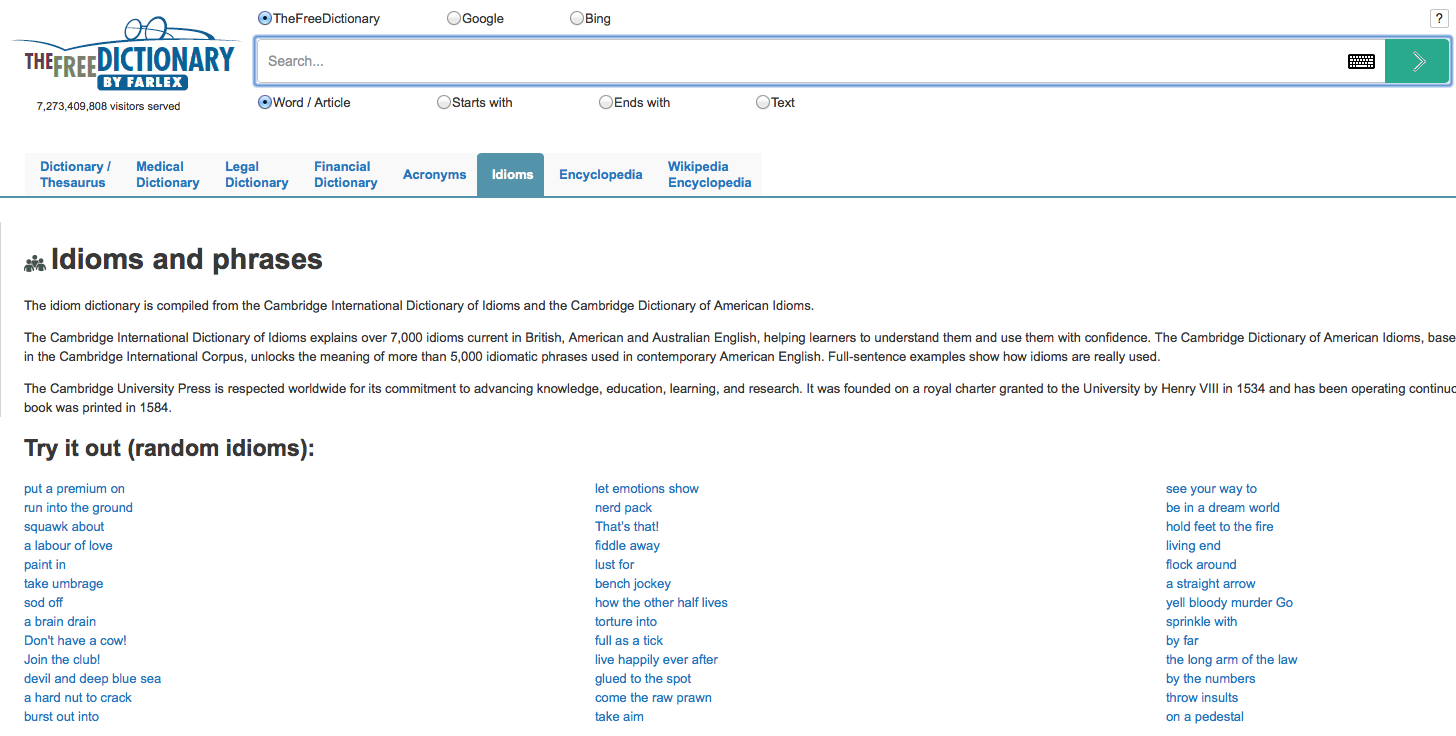
\includegraphics [clip, width=16cm]{./img/tryitout.png}
		\caption{Try\ it\ outのページ}
		\label{site:tryitout}
	\end{center}
	\end{figure}	

	\begin{figure}[htbp]
	\begin{center}
		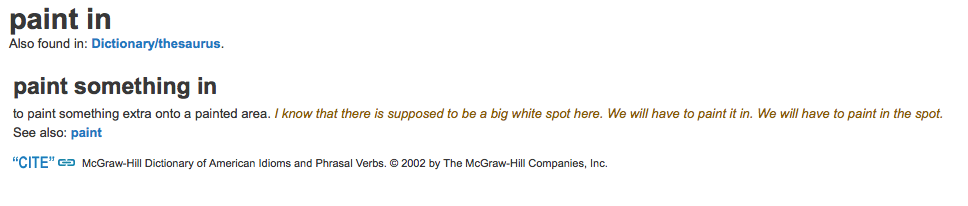
\includegraphics [clip, width=16cm]{./img/idiomsyousai.png}
		\caption{idiomの詳細ページ}
		\label{site:idiomsyousai}
	\end{center}
	\end{figure}	


\section{評価指標}
	本実験の評価を行った指標を以下に示す.ここで,実験の評価用データである50ペアのデータ集合を$T$, その要素となる各ペア\ $t \in T$\ について,
	\[
	\begin{cases}
		%\ q & :検索単語\\
		\ S^* & :正解パターンの集合\\
		\ S & :出力パターンの集合\\
		\ A\ (\subseteq S) & :Sのうち正解パターンと一致したパターンの集合\\
		\ c_{i}\ (\in S) &:Sのランク順に列挙されたパターン候補i番目が正解かどうか\\
		\ |P_{i}|\ (=\ \sum_{j=1}^{i} c_{i}) &:i番目までの正解と一致したパターン数
	\end{cases}
	\]
	とする.今回の実験では,イディオムの正解パターンを1つのみとしたため,すべてのtについて\ $|S^*|=1$\ となる.また,$c_{i}=1$でパターン候補i番目が正解パターンと一致,$c_{i}=0$で不一致とする.

	\subsection{単純適合率}
	単純な正解率として,各$t$について,$c_{i}=1$となる$c$が存在するか,すなわち出力パターン集合に正解パターンが含まれているか否か,をLを用いて
	\[
	L=\begin{cases}
		\ 0 & (|A| = 0)\\
		\ 1 & (|A| > 1)
	\end{cases}
	\]
	と表す.各$t$について$L$を算出し,$T$に関して平均する.

	\newpage
	\subsection{平均逆順位}
	\label{text:heikingyaku}
	平均逆順位は``MRR''と呼ばれ,本実験ではランクごとに列挙されたパターンのうち,最後に正解パターンと一致した順位までのすべての順位の逆数の和をとる.
	$$
	MRR=\frac{1}{|A|} \sum_{i=1}^n \frac{p_{i}}{i}
	$$
	ここで,「n:最後に正解パターンと一致したパターン候補の順位」とする.仮にパターン候補の1位,2位,5位が正解パターンと一致していた場合,
	$$
	MRR=\frac{1}{3}\ (\frac{1}{1} + \frac{1}{2} + \frac{1}{5}) \cong 0.567
	$$
	と計算することができる.このMRRを各ペア$t$について算出し,$T$に関して平均することで評価を行う.


	\subsection{平均適合率}
	平均適合率はAP(Average Precision)と呼ばれ,$S$のパターン候補1位からn位までの中に含まれる正解パターンと一致した数の平均値で与えられる.
	$$
	AP=\frac{1}{|A|} \sum_{i=1}^{n} p_{i} × \frac {|P_{i}|} {i}
	$$
	ここで,nは第\ref{text:heikingyaku}節と同様である.パターン候補の1位,2位,5位が正解パターンと一致していた場合,
	$$
	AP=\frac{1}{3} (\frac{1}{1} + \frac{2}{2} + \frac{3}{5}) \cong 0.867
	$$
	と計算できる.これも,各ペア$t$について算出し,$T$に関して平均する.


\newpage
\section{実験結果}
\label{text:kekka}
	以上の実験方法,および評価指標を用いて抽出できたパターンがどれほど正しいかを計算し,集合$T$に関して平均をとったところ
		$$
		L_{T}=0.84 \ \ 
		MRR_{T}=0.394\ \ 
		AP_{T}=0.838
		$$
	という結果を得ることが出来た.適合率である,$L$と$AP$に関してはかなり高い評価を得ることが出来た.これは,文章をコーパスから抜き出す際の検索語がイディオム全体となっているため,Queryとなるイディオムと用例が同じ文章を数多くコーパスから抜き出せたことが要因となっている.また,MRRについては,高い順位から低い順位まですべて正解パターンと一致していた場合,数値が低くなってしまうため,平均すると比較的低い結果となっている.\\



\section{パターン抽出例}

	入力となるコーパスから抜き出した文章,およびそこから抽出したパターン候補の例を図\ref{fig:bother_in},および図\ref{fig:bother_out}に示す.この例では,$Query="bother\ with"$,\ 正解パターンは$"bother\ with\ \sim" (〜のことを思い悩む)$である.\\
	 出力されたパターン候補のうち1位から5位までは``bother\ with$\sim$''という正解と一致するパターンを抽出することに成功している.6,7位のパターン候補に関しては,入力となった文章例にも存在する``bother''と``with''の間に別の単語を含んだ例文がノイズとなって抽出されていると考えられる.

	\begin{figure}[htbp]
	\begin{screen}
		・We didn't bother with lights.\\
		・We've found ourselves in a spot of bother with the police over at the office.\\
		・I am not going to bother with a certain group.\\
		・We didn't bother with that in the end.\\
		・But we can't bother with him any more now.\\
		・Well perhaps you wouldn't bother with that.\\
		・He would not bother himself with it now.\\
		・Well that lady don't bother with her next door down there.
	\end{screen}
	\caption{bother\ withの入力文章例}
	\label{fig:bother_in}
	\end{figure}


	\begin{figure}[htbp]
	\begin{center}
	\begin{minipage}{0.6\hsize}
	\begin{center}
	\begin{shadebox}
		1--bother,\ with,\ 【*/DT】 \\
		2--bother,\ with,\ 【*/NNS】 \\
		3--bother,\ with,\ 【*/PRP】 \\
		4--bother,\ with,\ the,\ 【*/NN】 \\
		5--bother,\ with,\ 【*/NN】 \\
		6--bother,\ 【*/PRP】 \\
		7--bother,\ 【*/IN】
	\end{shadebox}
	\end{center}
	\end{minipage}
	\end{center}
	\caption{bother\ withの抽出パターン候補}
	\label{fig:bother_out}
	\end{figure}

	\newpage
	抽出できたパターンの中には,「send\ {\it A}\ on\ {\it B}:AをBに送る,行かせる」,「represent\ {\it A}\ as\ {\it B}:AをBと描く,述べる」と言ったイディオムの単語間に穴あきの部分が存在するようなパターンについても抽出を行うことが出来た.図\ref{fig:anaaki}にそれぞれの抽出したパターン候補を示す.\\
	 ``send\ on''では1位のパターン候補のみ,``represent\ as''では1位と2位のパターン候補,が正解と一致している.数は少ないものの,穴あきのパターンという抽出することが難しいパターンを出力パターン候補のうちの上位で抽出することが出来ている.\\

	\begin{figure}[htbp]
	\begin{center}
	\begin{tabular}{c}
		\begin{minipage}{0.5\hsize}
		\begin{center}
		\begin{shadebox}
			1--send,\ 【*/PRP】,\ on,\ 【*/DT】\\
			2--send,\ to \\
			3--send,\ a,\ 【*/NN】 \\
			4--send,\ 【*/NN】\\
			5--send,\ 【*/DT】 \\
			6--send,\ 【*/IN】\\
			7--send,\ 【*/RP】 \\
			8--send,\ 【*/PRP】
		\end{shadebox}
		\hspace{2cm} (a)send\ on
		\end{center}
		\end{minipage}

		\begin{minipage}{0.5\hsize}
		\begin{center}
		\begin{shadebox}
			1--represent,\ the,\ 【*/NN】,\ as,\ 【*/DT'】\\
			2--represent,\ 【*/PRP】,\ as,\ 【*/DT】\\
			3--represent,\ 【*/NN】\\
			4--represent,\ 【*/DT】\\
			5--represent,\ 【*/NNP】\\
			6--represent,\ 【*/IN】
		\end{shadebox}
		\hspace{2cm} (b)represent as
		\end{center}
		\end{minipage}

	\end{tabular}
	\caption{穴あきパターンの例}
	\label{fig:anaaki}
	\end{center}
	\end{figure}

	 逆にパターンを抽出できなかった例としては,「appear\ for〜:〜(休んだ人の)代わりに現れる」などがあった.``appear\ for''に関して,入力となった文章の例を図\ref{fig:appear_in},抽出したパターン候補を図\ref{fig:appear_out},および作成されたSeqBDDの一部を図\ref{fig:appearfor}に示す.
	appear\ forの場合,コーパスから入力となる例文を抜き出す際にイディオムの単語間の距離を2単語まで許すという制約によって,appearとforの間に単語を含んだ文章を多く抜き出してしまったため,うまくパターンを取り出せていないことが分かった.これは,パターン抽出モジュールよりもコーパスから文章を抜き出すモジュールの改良が求められる.

	\newpage
	\begin{figure}
	\begin{screen}
		・Told me that one youth was in custody and another due to appear in court for the break−ins.\\
		・Wings appear externally for the first time and the insect takes on the appearance of an adult.\\
		・Even its two windows appear thatched, for they are fitted with wads of straw.\\
		・Their clicks are not FM, nor do they appear suitable for Doppler-shift speed metering.\\
		・They didn't appear to care for each other greatly.
	\end{screen}
	\caption{appear\ forの入力文章例}
	\label{fig:appear_in}
	\end{figure}

	 \\
	 \\

	\begin{figure}[htbp]
	\begin{center}
	\begin{minipage}{0.5\hsize}
	\begin{center}
	\begin{shadebox}
		1--appear,\ 【*/IN】,\ the,\ 【*/NN】\\
		2--appear,\ 【*/IN】,\ the,\ 【*/JJ】\\
		3--appear,\ 【*/JJ】\\
		4--appear,\ 【*/NN】,\ for\\
		5--appear,\ 【*/JJ】,\ for\\
		6--appear,\ to,\ 【*/VB】\\
		7--appear,\ 【*/RB】\\
		8--appear,\ 【*/TO】
	\end{shadebox}
	\end{center}
	\end{minipage}
	\end{center}
	\caption{appear\ forの抽出パターン候補}
	\label{fig:appear_out}
	\end{figure}

	\begin{figure}[htbp]
	\begin{center}
		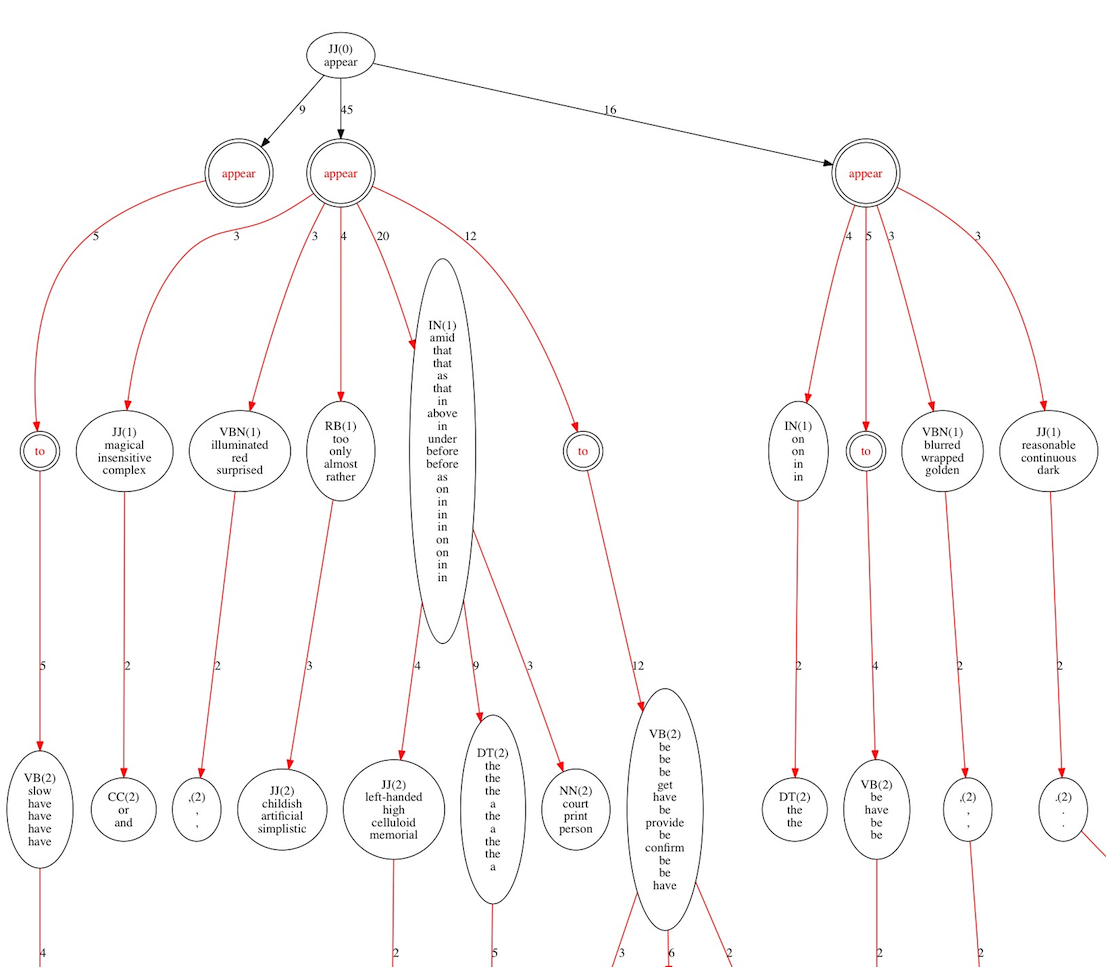
\includegraphics [clip, width=19cm, angle=90]{./img/appear_for.png}
		\caption{appear\ forで作成されたSeqBDDの一部}
		\label{fig:appearfor}
	\end{center}
	\end{figure}	


	\newpage
	\section{考察}
	\label{text:kousatu}
	\subsection{品詞タグ付の精度}
	現在は,文章からSeqBDDを構築する際に,まず入力となる文章それぞれについて構文解析エンジンを用いて各単語に品詞付を行っている.しかし,パターンを抽出できなかった``appear\ for''の例(図\ref{fig:appearfor})を見ると,まず根となる\ ``appear''\ の節点が複数に別れてしまっている.これは,構文解析の段階で,文章毎に``appear''が異なる品詞である,とタグ付けされているために生じている.そのため,品詞によって節点を作成する際に,本来同一であるべき根となる節点が複数個存在してしまい,その分枝が細かく別れてパターンの抽出を妨げていると考えられる.この場合,根となる節点のみに関しては,無条件で同一の節点であるとするという規約の元でSeqBDDを構築することで,無駄な枝分かれを防ぐことができ,パターン抽出精度の向上に繋がると考えられる.\\

	\subsection{節点圧縮の閾値}
	\label{text:assyuku_mondai}
	パターンを抽出する際に参照としている節点は,式(\ref{exp:sup_node})を満たした節点内のラベルが圧縮されたものである.ここで,より多くのパターンを抽出するために,式(\ref{exp:sup_node})の閾値を低くすることで,圧縮される節点の条件を緩くするという方法がある.これによって,いままでパターンとして表れていなかった新たなパターンも抽出することが可能になり,精度の上昇に繋がるかもしれない.しかし,ただ閾値を低くするだけでは,必要としない無駄なパターンの増加につながったり,節点のラベルに圧縮されるべき単語が2つ以上存在してしまうという新たな問題が生まれる可能性がある\footnote{例えば節点内の単語が2つのみの場合に,閾値を0.5以下にしてしまうと両方の単語ともに条件を満たすことになる}.そのため,パターンの抽出を最も効率よく行うことのできる閾値を調整して,調べる必要がある.

	\subsection{文章抜き出しモジュール}
	第\ref{text:kekka}節でも述べたように,パターンの取れなかったイディオムはほとんどがこの文章抜き出しに関する問題のためだった.
	現在の手法では,コーパスから文章を取ってくる際に,すべてのイディオムについて各単語の間に2単語までの距離を許している.そのために,本来のイディオムの用例でない文章も抜き出してしまい,その文章群がノイズとなってパターンの抽出を妨げている.\\
	\ \ この問題の一つの解決策としては,文章を抜き出す際のイディオムの単語間の距離の制約を,イディオム毎に変化させることが挙げられる.現在の仕様では,Queryとなるイディオムは穴あきのパターンとそうでないパターンが混在しており,その両パターンともに対応するために距離の制約を緩めていた.それを,穴あきのパターンの場合にはイディオムの単語間の距離を許し,そうでないパターンの場合には距離の制約を1単語も許さないようにすることで,パターンとして抽出できなかったイディオムについては改善が見込め,また既にパターンとして抽出できていたイディオムについては,より精度の高いパターンの抽出が望めるのではないだろうか.



\chapter{結論}
\label{text:ketsuron}

\section{まとめ}
本研究では,教師データを用いないテキストからのパターン抽出を,SeqBDDというデータ構造を用いて実現した.木構造を持つSeqBDDの末端部分を,同一な形のサブグラフの共有を行うことで,縮退することに成功し,巨大な量のテキストをよりコンパクトなデータ構造で表現することが可能となった.また,そこからパターンを抽出することで,出現頻度の高い単語の用例を獲得することができた.本稿では,特に構築したSeqBDDからパターンを抽出する手法の提案,および実装,さらにそれらの評価を行った.この提案手法の実現に伴って,大きく2つの処理モジュールを構築した.\\
 1つに,テキスト文章を入力とするSeqBDDの構築があった.節点の作成方法を吟味することで,よりパターンを抽出しやすい方法を導き,それらのプログラムの実装を行った.また,SeqBDDの大規模なデータ構造をコンパクトに表現することができる,という特徴を活かし,かつパターンを抽出しやすいように,節点ラベルの圧縮や枝切と言った,様々な方法によってデータ構造の加工を行った.\\
 もう1つに,構築したSeqBDDからパターンを抽出する処理があった.この処理では,提案手法によってパターンの抽出を行い易いデータ構造へと加工されているため,比較的単純なアルゴリズムによってパターンを抽出することが可能となった.\\
 また検証として,入力には,様々な文法パターンや用法を含む例文を備えた大規模電子データベース「British\ National\ Corpus」から抜き出した例文を,その例文を抜き出すための検索語,および正解データとなるイディオムのパターンを「TheFreeDictionary.com」というオンライン辞書サイトから収集し,上記の提案手法の実験,評価を行った.抽出できたイディオムのパターン候補と,サイトから収集した正解パターンの照合を行い,単純適合率($L$),平均逆順位($MRR$),平均適合率($AP$)という指標によって評価を行った.その結果,$L=0.84,\ MRR=0.394,\ AP=0.838$という値を得ることが出来た.平均順位を示すMRRに関しては,抽出したパターンの上位から下位までのすべてが正解パターンと一致するケースが多かったため,比較的低い数値となってしまったが,適合率を示すL,APに関しては8割を超えるというかなり高い評価を得ることが出来た.\\
 前述の考察(\ref{text:kousatu}節)でも述べたように,まだ様々な問題点,改善点を抱えている本研究ではあるが,SeqBDDを用いた教師なし手法による文からのパターン抽出の有用性を示せたのではないだろうか.

\section{今後の課題}
本研究における今後の課題としては,以下の様なものが挙げられる.

\subsection{既存のパターン抽出モジュールの改良}
第\ref{text:kousatu}節でも述べたが,既存のパターン抽出モジュールでは,
\begin{itemize}
	\item 品詞タグ付けの精度によって根となる節点が複数に分かれてしまい,それによって経路の細分化を招きパターン発見の難化を招いている
	\item パターンを抽出する際に,パターンかどうかの判定基準となる節点のラベル圧縮における最適な閾値を調べる必要がある
	\item 入力となる文書を抜き出すモジュールにが,パターン抽出を妨げるノイズとなる文章も一緒に抜き出してしまっている
\end{itemize}
といった改良点が挙げられる.これらの問題を改善していくことで,より精度の高いパターンの抽出を見込めるだろう.

\subsection{パターンの抽出方法}
現在のパターンの抽出方法は,節点のラベルが圧縮(第\ref{text:assyuku}節を参照)されているかどうか,という点に注目してその節点のラベルがパターンとなるかを判定している.しかし,考察(第\ref{text:kousatu}節)でも述べたが,節点のラベルを圧縮するために用いる閾値の問題がある.パターンを抽出するために最適な閾値を,様々なサンプルを通して発見することが望ましいが,発見できなかった場合には,検索語毎に適当な閾値に変更するなどの措置を取るか,抽出方法の変更を余儀なくされる可能性もある.


\subsection{与えられた語句の前半部分のパターン抽出}
今回の実験では,与えられた語句(イディオム)の後半部分のみについて,SeqBDDを構築しパターンの抽出を行った.しかし,与えられた単語の前後に共起しやすい単語,品詞のパターンを抽出することを目的としているため,前半部分についてもSeqBDDの構築,およびそこからのパターン抽出を行う必要がある.\\
\ \ 前半部分におけるパターン抽出は,後半とすべて同じ方法を用いるということは難しい.なぜなら,後半部分ではイディオムの前で文を区切り,それ以降の文章を入力としてSeqBDDを構築したため,根となる節点のラベルは必ずイディオムの先頭語であり,その先頭語の節点から各経路を辿って行き,パターンの判定を行うことが可能であった.しかし,前半部分では,根となる節点は各文章の先頭語であり,もちろん同じ単語,品詞であるとは言えない.そのため,根付近のサブグラフに関して細かい枝分かれが発生することになる.終端節点付近では,イディオムの直近となるため比較的似た単語や品詞が現れる際には,節点の共有が行われパターンとして抽出することができるが,根の付近の枝分かれにより,経路がより細かく別れるため,パターン発見の難化に繋がるのではないかと考えられる.


\subsection{検索単語の抽象化と正解パターン集合の拡大}
今回の実験は,検索単語はイディオム全体,正解パターンは1種のみという限定された範囲内で行った.しかし,現在の目標の一つとして,ある単語(1つ,または複数)が与えられた際に,その単語の前後に出現しやすい単語や品詞をパターン候補として利用者に提供するというシステムの構築がある.この実現に向けて,まず,行うべきことが,前述した単語の前半部分のパターン抽出,さらに,例えばイディオムの先頭語のみで文章を抜き出してくると言った,より抽象的な表現の検索単語を用いてSeqBDDを構築することである.それに対応して,正解となるパターンの数も増やし,再度実験,評価を行う必要がある.

\newpage
\acknowledgment
本研究を進めるにあたり,多大なるご指導ご支援を頂きました九州大学大学院システム情報科学研究院の田中久美子教授に深く感謝の意を表します.
最後に,本研究において様々なご協力をいただきました田中研究室の皆様方に深く感謝し,お礼を申し上げます.

\bibliographystyle{junsrt}
\bibliography{thesis}

\appendix
\end{document}